\documentclass[journal=jcp,manuscript=suppinfo]{achemso}
\setkeys{acs}{maxauthors=0,articletitle=true}

%%%%%%%%%%%%%%%%%%%%%%%%%%%%%%%%%%%%%%%%%%

\usepackage{achemso}
\usepackage{graphics}
\usepackage{amssymb,amsfonts}
\usepackage{graphicx}
\usepackage[table]{xcolor}
\usepackage{threeparttable}
\usepackage{multirow}
\usepackage{caption}
\usepackage{subcaption}
\usepackage{booktabs}
\usepackage{colortbl}
\usepackage{amsmath}
\usepackage{amsopn}
\usepackage{siunitx}
\usepackage{bm}
\usepackage{color}
\usepackage{array}
\usepackage{lscape}
\usepackage{mciteplus}
\usepackage[version=3]{mhchem}
\usepackage{ulem}
\usepackage{listings}
\usepackage{enumerate}
\usepackage{makecell}

\captionsetup{labelfont=bf}
\SectionNumbersOn
\renewcommand{\thefootnote}{\fnsymbol{footnote}}
\newlength{\wordwidth}

%%%%%%%%%%%%%%%%%%%%%%%%%%%%%%%%%%%%%%%%%%

\author{Janus J. Eriksen}
\email{janus.eriksen@bristol.ac.uk}
\affiliation{School of Chemistry, University of Bristol, Cantock's Close, Bristol BS8 1TS, United Kingdom}
%
\author{Tyler A. Anderson}
\affiliation{Laboratory of Atomic and Solid State Physics, Cornell University, Ithaca, New York 14853, USA}
\author{J. Emiliano Deustua}
\affiliation{Department of Chemistry, Michigan State University, East Lansing, MI 48824, USA}
\author{Khaldoon Ghanem}
\affiliation{Max-Planck-Institut f{\"u}r Festk{\"o}rperforschung, 70569 Stuttgart, Germany}
\author{Diptarka Hait}
\affiliation{Kenneth S. Pitzer Center for Theoretical Chemistry, Department of Chemistry, University of California, Berkeley, California 94720, USA}
\alsoaffiliation{Chemical Sciences Division, Lawrence Berkeley National Laboratory, Berkeley, California 94720, USA}
\author{Mark R. Hoffmann}
\affiliation{Chemistry Department, University of North Dakota, Grand Forks, ND 58202-9024, USA}
\author{Seunghoon Lee}
\affiliation{Division of Chemistry and Chemical Engineering, California Institute of Technology, Pasadena, California 91125, USA}
\author{Daniel S. Levine}
\affiliation{Kenneth S. Pitzer Center for Theoretical Chemistry, Department of Chemistry, University of California, Berkeley, California 94720, USA}
\author{Ilias Magoulas}
\affiliation{Department of Chemistry, Michigan State University, East Lansing, MI 48824, USA}
\author{Jun Shen}
\affiliation{Department of Chemistry, Michigan State University, East Lansing, MI 48824, USA}
\author{Norman M. Tubman}
\affiliation{Kenneth S. Pitzer Center for Theoretical Chemistry, Department of Chemistry, University of California, Berkeley, California 94720, USA}
\author{K. Birgitta Whaley}
\affiliation{Kenneth S. Pitzer Center for Theoretical Chemistry, Department of Chemistry, University of California, Berkeley, California 94720, USA}
\author{Enhua Xu}
\affiliation{Graduate School of Science, Technology, and Innovation, Kobe University, 1-1 Rokkodai-cho, Nada-ku, Kobe 657-8501, Japan}
\author{Yuan Yao}
\affiliation{Laboratory of Atomic and Solid State Physics, Cornell University, Ithaca, New York 14853, USA}
\author{Ning Zhang}
\affiliation{Beijing National Laboratory for Molecular Sciences, Institute of Theoretical and Computational Chemistry, College of Chemistry and Molecular Engineering, Peking University, Beijing 100871, China}
%
\author{Ali Alavi}
\email{a.alavi@fkf.mpg.de}
\affiliation{Max-Planck-Institut f{\"u}r Festk{\"o}rperforschung, 70569 Stuttgart, Germany}
\alsoaffiliation{Department of Chemistry, University of Cambridge, Cambridge CB2 1EW, United Kingdom}
\author{Garnet Kin-Lic Chan}
\email{gkc1000@gmail.com}
\affiliation{Division of Chemistry and Chemical Engineering, California Institute of Technology, Pasadena, California 91125, USA}
\author{Martin Head-Gordon}
\email{mhg@cchem.berkeley.edu}
\affiliation{Kenneth S. Pitzer Center for Theoretical Chemistry, Department of Chemistry, University of California, Berkeley, California 94720, USA}
\alsoaffiliation{Chemical Sciences Division, Lawrence Berkeley National Laboratory, Berkeley, California 94720, USA}
\author{Wenjian Liu}
\email{liuwj@sdu.edu.cn}
\affiliation{Qingdao Institute for Theoretical and Computational Sciences, Shandong University, Qingdao, Shandong 266237, China}
\author{Piotr Piecuch}
\email{piecuch@chemistry.msu.edu}
\affiliation{Department of Chemistry, Michigan State University, East Lansing, MI 48824, USA}
\alsoaffiliation{Department of Physics and Astronomy, Michigan State University, East Lansing, MI 48824, USA}
\author{Sandeep Sharma}
\email{sandeep.sharma@colorado.edu}
\affiliation{Department of Chemistry, The University of Colorado at Boulder, Boulder, Colorado 80302, USA}
\author{Seiichiro L. Ten-no}
\email{tenno@garnet.kobe-u.ac.jp}
\affiliation{Graduate School of Science, Technology, and Innovation, Kobe University, 1-1 Rokkodai-cho, Nada-ku, Kobe 657-8501, Japan}
\author{C. J. Umrigar}
\email{cyrusumrigar@gmail.com}
\affiliation{Laboratory of Atomic and Solid State Physics, Cornell University, Ithaca, New York 14853, USA}
\author{J{\"u}rgen Gauss}
\email{gauss@uni-mainz.de}
\affiliation{Department Chemie, Johannes Gutenberg-Universit{\"a}t Mainz, Duesbergweg 10-14, 55128 Mainz, Germany}

\renewcommand*\titlesize{\Large}
\renewcommand*\authorsize{\small}
\renewcommand*\affilsize{\footnotesize}
\renewcommand*\emailsize{\scriptsize}

%%%%%%%%%%%%%%%%%%%%%%%%%%%%%%%%%%%%%%%%%%

\title[TITLE]{The Ground State Electronic Energy of Benzene}

%%%%%%%%%%%%%%%%%%%%%%%%%%%%%%%%%%%%%%%%%%

\begin{document}
%

\newpage

\section{Geometry}

The geometry of benzene used in our study is the MP2/6-31G$^{\ast}$ optimized structure from Ref. \citenum{sauer_thiel_cc3_benchmark_jcp_2008}, cf. Table \ref{geometry_SI_table}. For reference, the nuclear repulsion and Hartree-Fock energies are $E_{\text{nuc}} = 203.15350971$ $E_{\text{H}}$ and $E_{\text{HF}} = -230.721819131$ $E_{\text{H}}$, respectively.
%
\begin{table}[ht]
\begin{center}
\caption{C$_6$H$_6$ (in \AA).}
\label{geometry_SI_table}
\begin{tabular}{c|rrr}
\toprule
\multicolumn{1}{c|}{Atom} & \multicolumn{1}{c}{$x$} & \multicolumn{1}{c}{{\textbf{$y$}}} & \multicolumn{1}{c}{{\textbf{$z$}}} \\
\midrule\midrule
C & $0.000000$ & $1.396792$ & $0.000000$ \\
C & $0.000000$ & $-1.396792$ & $0.000000$ \\
C & $1.209657$ & $0.698396$ & $0.000000$ \\
C & $-1.209657$ & $-0.698396$ & $0.000000$ \\
C & $-1.209657$ & $0.698396$ & $0.000000$ \\
C & $1.209657$ & $-0.698396$ & $0.000000$ \\
H & $0.000000$ & $2.484212$ & $0.000000$ \\
H & $2.151390$ & $1.242106$ & $0.000000$ \\
H & $-2.151390$ & $-1.242106$ & $0.000000$ \\
H & $-2.151390$ & $1.242106$ & $0.000000$ \\
H & $2.151390$ & $-1.242106$ & $0.000000$ \\
H & $0.000000$ & $-2.484212$ & $0.000000$ \\
\midrule
\end{tabular}
\vspace{-1.4cm}
\end{center}
\end{table}
%

\section{Main Results}

Table \ref{results_SI_table} summarizes the results in Fig. 1 of the main study. Methods are ordered by the final correlation energy.
%
\begin{table}[ht]
\begin{center}
\caption{Summary of Fig. 1 from the main study.}
\label{results_SI_table}
\begin{tabular}{l|r}
\toprule
\multicolumn{1}{c|}{Method} & \multicolumn{1}{c}{$\Delta E$/m$E_{\text{H}}$} \\
\midrule\midrule
ASCI & $-860.0$ \\
iCI & $-861.1$ \\
CCSDTQ & $-862.4$ \\
DMRG & $-862.8$ \\
FCCR & $-863.0$ \\
MBE-FCI & $-863.0$ \\
CAD-FCIQMC & $-863.4$ \\
AS-FCIQMC & $-863.7$ \\
SHCI & $-864.2$ \\
\midrule
\end{tabular}
\vspace{-1.4cm}
\end{center}
\end{table}
%

\section{MBE-FCI}

%
\begin{figure}[ht!]
\begin{center}
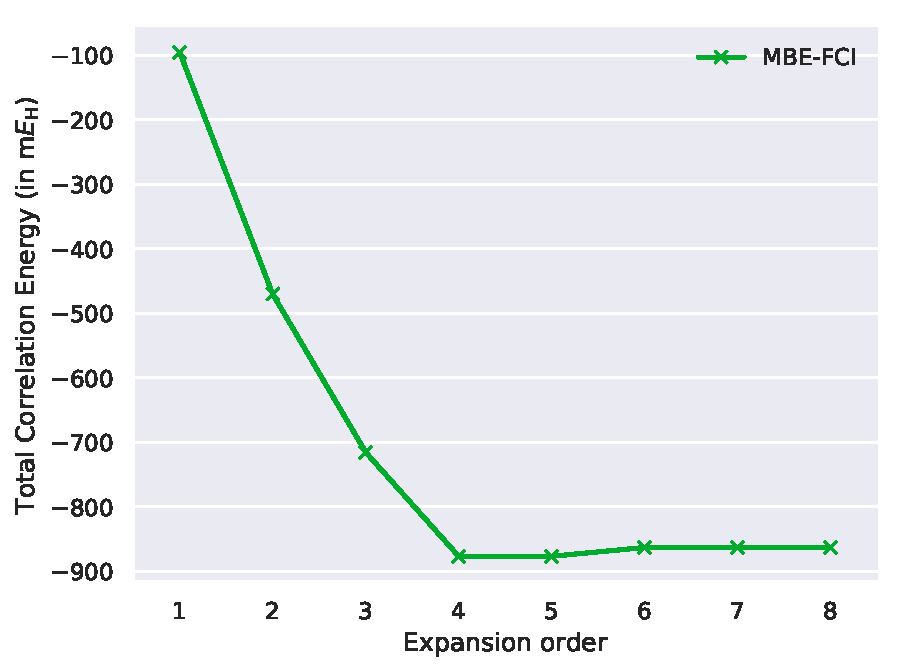
\includegraphics[scale=0.75]{figures/mbe_fci/mbe_fci.pdf}
\caption{MBE-FCI results.}
\label{mbe_fci_SI_fig}
\end{center}
\vspace{-0.6cm}
\end{figure}
%
In MBE-FCI theory~\cite{eriksen_mbe_fci_jpcl_2017,eriksen_mbe_fci_weak_corr_jctc_2018,eriksen_mbe_fci_strong_corr_jctc_2019,eriksen_mbe_fci_general_jpcl_2019}, the complete set of MOs for a given system is divided into a reference and an expansion space. An MBE-FCI expansion in the latter of these space hence recovers the residual correlation not captured by an FCI calculation constrained to the former. The MBE-FCI calculation of the present work is presented in Figure \ref{mbe_fci_SI_fig}, as performed in an embarrassingly parallel manner using the open-source {\texttt{PyMBE}} code~\cite{pymbe} on Intel Xeon E5-2697v4 (Broadwell) hardware (36 cores $@$ 2.3 GHz, 3.56 GB/core). The calculation was performed in a basis of localized Pipek-Mezey MOs~\cite{pipek_mezey_jcp_1989} with a ($6e$,$6$o) reference space consisting of the $\pi$- and $\pi^{\ast}$-orbitals and electrons. The final correlation energy is $\Delta E_{\text{MBE-FCI}} = -863.03$ m$E_{\text{H}}$.\\

In the course of preparing the code for running high-accuracy MBE-FCI calculations on the benzene molecule, a new screening protocol was implemented. At each order, MOs are screened away from the full expansion space according to their relative (absolute) magnitude, which in turn leads to a reduced number of increment calculations at the orders to follow. Specifically, only the MOs of the expansion space (at any given order) that give rise to the numerically largest increments will be retained at the following order. For the calculation of the present work, the percentages of the expansion space retained ($a_{\text{retain}}$) alongside the number of individual CASCI calculations at any given order ($K_{\text{CASCI}}$) are presented in Table \ref{mbe_fci_SI_table}. In addition, a number of optimizations were made to the code base. Most crucially, a new pruning scheme was introduced to make sure that only non-redundant increments are stored in memory throughout the total MBE-FCI calculation. For instance, once the $i$th MO gets screened away from the expansion space, all increments at lower orders, which reference this MO, are not needed anymore and may thus be pruned. This allows for significantly larger problem sizes to be treated by the method. As such, the limiting factor in converging MBE-FCI even tighter for the problem at hand, that is, screening less throughout the expansion, is related to available computer ressources rather than physical memory.
%
\begin{table}[ht]
\begin{center}
\caption{MBE-FCI calculation details.}
\label{mbe_fci_SI_table}
\begin{tabular}{l|r|r|r}
\toprule
\multicolumn{1}{c|}{Order} & \multicolumn{1}{c|}{$a_{\text{retain}}/\%$} & \multicolumn{1}{c|}{$\Delta E$/m$E_{\text{H}}$} & \multicolumn{1}{c}{$K_{\text{CASCI}}$} \\
\midrule\midrule
1 & 100.0 & $-95.1132$ & 102 \\
2 & 100.0 & $-469.884$ & 5,151 \\
3 & 100.0 & $-715.265$ & 171,700 \\
4 & 100.0 & $-876.637$ & 4,249,575 \\
5 & 100.0 & $-876.624$ & 83,291,670 \\
6 & 50.0 & $-862.988$ & 1,346,548,665 \\
7 & 25.0 & $-863.027$ & 115,775,100 \\
8 & 12.5 & $-863.027$ & 495 \\
\midrule
\end{tabular}
\vspace{-1.4cm}
\end{center}
\end{table}
%

\section{DMRG}

For details on DMRG theory, please see a number of contemporary reviews on the topic~\cite{chan_dmrg_2011,wouters_dmrg_2014,knecht_dmrg_2016}. All DMRG calculations were performed using an unmodified version of the {\texttt{BLOCK}} code (v1.5)~\cite{chan_head_gordon_dmrg_jcp_2002,chan_dmrg_jcp_2004,chan_polyacetylenes_jcp_2008,sharma_chan_dmrg_2012,chan_dmrg_2015}, executed through the {\texttt{PySCF}} program~\cite{pyscf_prog,pyscf_wires_2018,pyscf_jcp_2020}, on Intel Xeon CPU E5-2680v4 (28-36 cores $@$ 2.4 GHz, 9.85 GB/core) and Xeon Gold 6130 (32 cores $@$ 2.1 GHz, 6.0 GB/core) nodes. Calculations were run in parallel on 100-200 cores. Maximum total memory usage was estimated at 1.15 Tb in total across all cores; this includes
replicated data on the cores. We used the standard procedures described in Ref. \citenum{chan_dmrg_2015}, including (i) Edminston-Ruedenberg split-localization of orbitals~\cite{edmiston_ruedenberg_rev_mod_phys_1963}, (ii) and the use of the genetic algorithm option in \texttt{BLOCK} to order the orbitals. The forward schedule was carried out up to a maximum bond dimension of $M=7000$, then the backward schedule was carried out to obtain fully converged results for extrapolation back down to $M=1000$.
We obtained our initial integral file from the Umrigar group for the blind challenge and used these for the DMRG calculations.
As we found out subsequently, the integral file corresponded to optimized SHCI orbitals. As this makes the results more complicated to reproduce,
we provide the full integral file at \url{https://github.com/seunghoonlee89/SI-benzene-paper-DMRG}. We also
verified on some smaller runs that using CCSD natural orbitals gave similar energies. The results from the backwards schedule of DMRG are listed in table~\ref{tab:DMRG_reverse}.\\

%
\begin{table}[ht]
\begin{center}
\caption{DMRG correlation energy ($E$ in m$E_{\text{H}}$) and discarded weights ($w$) with the backwards schedule.}
\label{tab:DMRG_reverse}
\begin{tabular}{cccccccc}
\toprule
$M$ & $1000$               & $2000$               & $3000$               & $4000$               & $5000$                & $6000$                & $\infty$    \\ \midrule\midrule
$w$ & $5.3 \times 10^{-5}$ & $2.9 \times 10^{-5}$ & $2.1 \times 10^{-5}$ & $1.6 \times 10^{-5}$ & $1.3 \times 10^{-5}$  & $1.0 \times 10^{-5}$  &             \\
$E$ & $-844.9$ 		   & $-852.9$  		  & $-855.9$ 		 & $-857.5$ 		& $-858.5$ 		& $-859.2$		& $-862.8(7)$ \\
\midrule
\end{tabular}
\vspace{-0.6cm}
\end{center}
\end{table}
%
DMRG yields two separate results: a variational upper bound and an extrapolated number based on the different bond dimensions. The lowest variational correlation energy is $\Delta E_{\text{DMRG(var)}} = -859.5$ m$E_{\text{H}}$, corresponding to the $M=7000$ result from the partially converged forwards schedule. The linear extrapolation was based on using the fully converged backwards schedule results for $M=6000$ to $M=1000$ (the variational $M=6000$ result was $-859.2$ m$E_{\text{H}}$) giving a final number of $\Delta E_{\text{DMRG}(\infty)} = -862.8$ m$E_{\text{H}}$, cf. Figure \ref{dmrg_SI_fig}. The standard practice in DMRG for estimating an error from the extrapolation is to report a fraction of the extrapolation distance, typically $1/5$. Here, the estimate ($1/5$ extrapolation distance error metric) is $0.7$ m$E_{\text{H}}$. The error of the linear fit (std. dev. of the intercept) is about $0.2$ m$E_{\text{H}}$, suggesting the 1/5 extrapolation distance error is an overestimate.
%
\begin{figure}[ht!]
\begin{center}
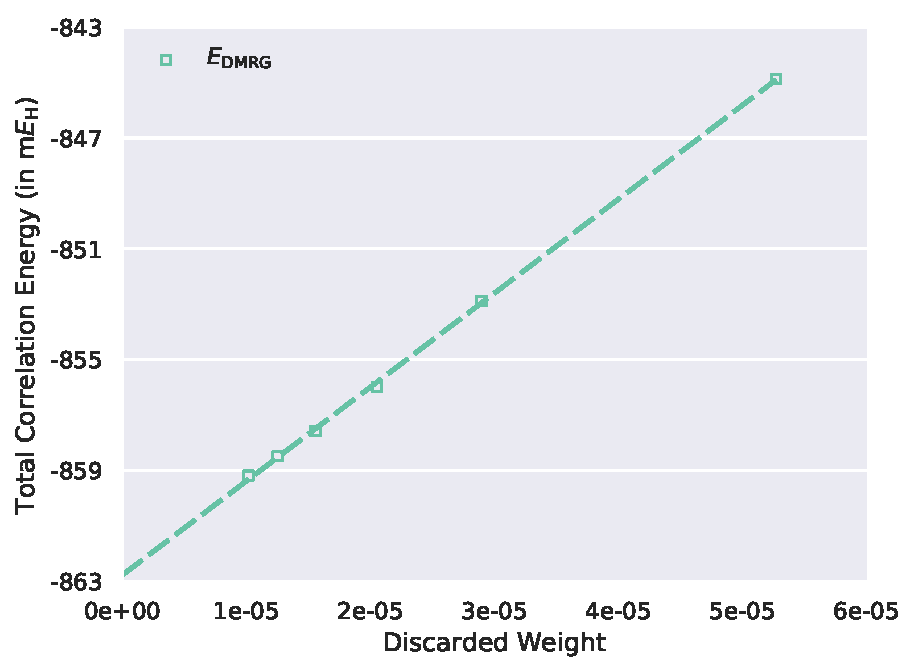
\includegraphics[scale=0.75]{figures/dmrg/dmrg.pdf}
\caption{DMRG results.}
\label{dmrg_SI_fig}
\end{center}
\end{figure}
%

\section{AS-FCIQMC}\label{as_fciqmc_SI_sect}

For details on the adaptive shift formalism, please see Ref. \citenum{ghanem_alavi_fciqmc_jcp_2019}. All AS-FCIQMC calculations were performed using the {\texttt{NECI}} code~\cite{neci,neci_jcp_2020} in parallel on Intel Xeon CPU E5-2698v4 nodes (40 cores $@$ 2.2 GHz, 6.4 GB/core). The orbitals used were those of a preceding RHF orbitals and the FCIQMC runs were performed in a basis of pure Slater determinants (no spin adaptation). Following an equilibration run with $\num{1.e8}$ walkers (yielding a correlation energy of $\Delta E_{\text{AS-FCIQMC(init)}} = -863.3\pm0.9$ m$E_{\text{H}}$), a first calculation with $\num{1.e9}$ (1B) walkers (growing from $\num{1.e8}$) yielded a correlation energy $\Delta E_{\text{AS-FCIQMC(1B)}} = -864.8\pm0.5$ m$E_{\text{H}}$. Next, a second calculation with $\num{2.e9}$ (2B) walkers (growing from $\num{1.e9}$) resulted in a correlation energy of $\Delta E_{\text{AS-FCIQMC(2B)}} = -863.7\pm0.3$ m$E_{\text{H}}$. The stochastic error bar of $0.3$ m$E_{\text{H}}$ is derived by averaging over the last 2637 time steps (discarding the first 5000 time steps for walker growth and equilibration period), and doing a blocking analysis. The AS‐FCIQMC(2B) result is used in Fig. 1 of the main study. For the largest AS-FCIQMC calculations (2B), the {\texttt{NECI}} code used 2.6 GB/core, i.e., 3162 Gb in total distributed over 32 nodes (40 cores/node).

%%%%% PIECUCH's SECTION, 24 JULY 2020 %%%%%

\section{CAD-FCIQMC}
\label{cad_fciqmc_SI_sect}

The CAD-FCIQMC approach, introduced in Ref.\ \citenum{piecuch_monte_carlo_cc_jcp_2018}, belongs to a new category
of semi-stochastic methods, in which information about higher-order wave function components extracted from
the FCIQMC \cite{piecuch_Booth2009,piecuch_Cleland2010,ghanem_alavi_fciqmc_jcp_2019}
or CCMC \cite{piecuch_Thom2010,piecuch_Franklin2016}
propagations is read into deterministic CC computations.
\cite{piecuch_monte_carlo_cc_prl_2017,piecuch_monte_carlo_cc_jcp_2018,piecuch_monte_carlo_eom_cc_jcp_2019,%
piecuch_monte_carlo_eom_cc_mp_2020}
CAD-FCIQMC can also be classified as an externally corrected CC method.
\cite{piecuch_extcc_1,piecuch_extcc_2,piecuch_extcc_3,piecuch_extcc_4,piecuch_extcc_5,%
piecuch_extcc_6,piecuch_extcc_7,piecuch_extcc_8,piecuch_extcc_9}
We recall that all externally corrected CC approaches are based on the observation that as long as the
Hamiltonian does not contain higher--than--two-body interactions, the CC amplitude equations projected
on the singly and doubly excited determinants, in which no approximations are made, do not engage
higher--than--four-body components of the cluster operator $T$. Thus, by solving these equations for the
singly and doubly excited clusters, $T_{1}$ and $T_{2}$, respectively, in the presence of their exact triply
($T_{3}$) and quadruply ($T_{4}$) excited counterparts extracted from FCI, one obtains the exact
$T_{1}$ and $T_{2}$ and the exact correlation energy, which is given by the expression
\begin{equation}
\Delta E = \langle \Phi | \left[ H_{N} \exp(T_{1} + T_{2}) \right]_{C} |\Phi\rangle ,
\label{eq-cad4}
\end{equation}
where $H_{N} = H - \langle \Phi | H | \Phi \rangle$ is the
Hamiltonian in the normal-ordered form relative to the reference determinant $|\Phi \rangle$
and the subscript $C$ designates the connected operator product. This means that by using a well-behaved
source of the $T_{3}$ and $T_{4}$ clusters, capable of offering their accurate description for the $N$-electron
system of interest, one can obtain
highly accurate $T_{1}$, $T_{2}$, and $\Delta E$. In the case of CAD-FCIQMC, this well-behaved source
is the FCIQMC wave function $|\Psi^{\rm (MC)}(\tau)\rangle$ obtained at a sufficiently long propagation time $\tau$,
which converges to the corresponding FCI ground state as $\tau$ approaches $\infty$.

In order to extract the desired triply and quadruply excited clusters from the FCIQMC
state $|\Psi^{\rm (MC)}(\tau)\rangle$,
we rewrite it to satisfy the intermediate normalization as
\begin{equation}
|\Psi^{\rm (MC)}(\tau)\rangle = [1 + C^{\rm (MC)}(\tau)] |\Phi\rangle
\equiv \left[1 + \sum_{n=1}^{N} C_{n}^{\rm (MC)}(\tau)\right] |\Phi\rangle,
\label{eq-cad1}
\end{equation}
where $C_{n}^{\rm (MC)}(\tau)$ are the CI excitation operators determined by counting walkers
at the $n$-tuply excited determinants contributing to $|\Psi^{\rm (MC)}(\tau)\rangle$ (dividing
the numbers of these walkers by the number of walkers at $|\Phi\rangle$), replace Eq.\ (\ref{eq-cad1}) by the
equivalent exponential ansatz,
\begin{equation}
|\Psi^{\rm (MC)}(\tau)\rangle = \exp[T^{\rm (MC)}(\tau)] |\Phi\rangle
\equiv \exp \left[\sum_{n=1}^{N} T_{n}^{\rm (MC)}(\tau)\right] |\Phi\rangle ,
\label{eq-cad2}
\end{equation}
where $T^{\rm (MC)}(\tau)$ is defined as $\ln [1 +  C^{\rm (MC)}(\tau)]$,
and exploit the resulting relationships between the CI excitation operators $C_{n}^{\rm (MC)}(\tau)$
and their CC counterparts $T_{n}^{\rm (MC)}(\tau)$ (see Ref.\ \citenum{piecuch_monte_carlo_cc_jcp_2018}).
Assuming that $|\Psi^{\rm (MC)}(\tau)\rangle$ converges to the FCI wave function as $\tau$ increases,
by solving the CC amplitude equations projected on the singly and doubly excited determinants,
$|\Phi_{i}^{a}\rangle$ and $|\Phi_{ij}^{ab}\rangle$, respectively, in which
$T_{3}$ and $T_{4}$ are replaced by their $T_{3}^{\rm (MC)}(\tau)$ and $T_{4}^{\rm (MC)}(\tau)$
counterparts obtained from the cluster analysis of $|\Psi^{\rm (MC)}(\tau)\rangle$, i.e.,
\begin{equation}
\begin{split}
\langle \Phi_{i}^{a} | \left[ H_{N} \exp(T_{1} + T_{2} + T_{3}^{\rm (MC)}(\tau)) \right]_{C} |\Phi\rangle & = 0, \\
\langle \Phi_{ij}^{ab} | \left[H_{N} \exp(T_{1} + T_{2} + T_{3}^{\rm (MC)}(\tau)
+ T_{4}^{\rm (MC)}(\tau))\right]_{C} |\Phi\rangle & = 0,
\end{split}
\label{eq-cad3}
\end{equation}
for the singly and doubly excited clusters $T_{1}$ and $T_{2}$, we are guaranteed to obtain
the exact $T_{1}$ and $T_{2}$ and thus the exact, FCI, correlation energy
in the $\tau = \infty$ limit. In other
words, if the walker population and propagation time $\tau$ used to generate the FCIQMC
state $|\Psi^{\rm (MC)}(\tau)\rangle$ are large enough, so that $T_{3}^{\rm (MC)}(\tau)$
and $T_{4}^{\rm (MC)}(\tau)$ extracted from $|\Psi^{\rm (MC)}(\tau)\rangle$
and $T_{1}$ and $T_{2}$ obtained by solving the CC system defined by Eq.\ (\ref{eq-cad3})
are good approximations to their exact, FCI or FCC, values,
the CAD-FCIQMC correlation energy calculated using Eq.\ (\ref{eq-cad4}) is anticipated
to be a very accurate approximation to its FCI counterpart. The numerical evidence
reported in Ref.\ \citenum{piecuch_monte_carlo_cc_jcp_2018}
shows that this is indeed the case. It is worth noting
that one does not have to process the entire FCIQMC wave function $|\Psi^{\rm (MC)}(\tau)\rangle$
to determine $T_{3}^{\rm (MC)}(\tau)$ and $T_{4}^{\rm (MC)}(\tau)$ entering
Eq.\ (\ref{eq-cad3}); all one needs to know are the CI excitation amplitudes through
quadruples defining the $C_{n}^{\rm (MC)}(\tau)$ operators with $n = \mbox{1--4}$.

As shown in Ref.\ \citenum{piecuch_monte_carlo_cc_jcp_2018}, by considering the CC system given by Eq.\ (\ref{eq-cad3})
and by solving it for $T_{1}$ and $T_{2}$ deterministically, the CAD-FCIQMC approach can substantially
accelerate the purely stochastic FCIQMC calculations. It also offers an interesting diagnostic of the quality
of the instantaneous FCIQMC wave function $|\Psi^{\rm (MC)}(\tau)\rangle$ obtained at a given time $\tau$,
especially of its $C_{n}^{\rm (MC)}(\tau)$ components through $n=4$, using computational steps that are
similar to those characterizing the conventional CCSD method\cite{piecuch_ccsd}
once the cluster analysis of $|\Psi^{\rm (MC)}(\tau)\rangle$, needed to determine
$T_{3}^{\rm (MC)}(\tau)$ and $T_{4}^{\rm (MC)}(\tau)$, is completed.
The latter feature is particularly useful in the context
of the present study. Indeed, if in the process of solving the CC amplitude equations defined
by Eq.\ (\ref{eq-cad3}) the $T_{1}$ and $T_{2}$ clusters significantly relax compared to their initial
$T_{1}^{\rm (MC)}(\tau)$ and $T_{2}^{\rm (MC)}(\tau)$ values extracted from
%%%%% the FCIQMC wave function
$|\Psi^{\rm (MC)}(\tau)\rangle$, so that the final CAD-FCIQMC correlation energy $\Delta E$,
calculated using Eq.\ (\ref{eq-cad4}),
is considerably different than its instantaneous FCIQMC counterpart determined at time $\tau$,
\begin{equation}
\begin{split}
\Delta E^{\rm (MC)}
& = \langle \Phi | H_{N} \left[ C_{1}^{\rm (MC)}(\tau) + C_{2}^{\rm (MC)}(\tau) \right] |\Phi\rangle \\
& = \langle \Phi | \left[ H_{N} \exp(T_{1}^{\rm (MC)}(\tau) + T_{2}^{\rm (MC)}(\tau)) \right]_{C} |\Phi\rangle ,
\end{split}
\label{eq-cad5}
\end{equation}
we can conclude that the FCIQMC wave function $|\Psi^{\rm (MC)}(\tau)\rangle$
is not well converged yet. On the other hand,
if $T_{3}^{\rm (MC)}(\tau)$ and $T_{4}^{\rm (MC)}(\tau)$ obtained by the cluster analysis of
$|\Psi^{\rm (MC)}(\tau)\rangle$ are nearly exact, $T_{1}$, $T_{2}$, and $\Delta E$
will relax very little during the CC iterations based on Eq.\ (\ref{eq-cad3}) compared
to their $T_{1}^{\rm (MC)}(\tau)$, $T_{2}^{\rm (MC)}(\tau)$, and $\Delta E^{\rm (MC)}$ values.
This means that if the final CAD-FCIQMC correlation energy $\Delta E$, Eq.\ (\ref{eq-cad4}), obtained
after solving the CC system defined by Eq.\ (\ref{eq-cad3}), and its initial FCIQMC counterpart
$\Delta E^{\rm (MC)}$, Eq.\ (\ref{eq-cad5}), agree to within a certain numerical precision, we may be able to
claim that the CAD-FCIQMC estimate of the correlation energy is stable to within the same precision.
This follows the observation, which is a formal basis of all externally corrected CC approaches, that if
$T_{3}^{\rm (MC)}(\tau)$ and $T_{4}^{\rm (MC)}(\tau)$ were exact, $T_{1}$ and $T_{2}$ obtained by solving
Eq.\ (\ref{eq-cad3}) would become exact too, i.e., the relaxation of $T_{1}$, $T_{2}$, and $\Delta E$ compared
to their $T_{1}^{\rm (MC)}(\tau)$, $T_{2}^{\rm (MC)}(\tau)$, and $\Delta E^{\rm (MC)}$ values would be zero.

The deterministic {\it a posteriori} CAD-FCIQMC steps, as summarized above, may provide useful insights
into the error bounds associated with the FCIQMC wave functions, but this is not to say that these
steps alone provide complete information about errors. In analyzing the results of CAD-FCIQMC calculations,
we have to keep in mind that the underlying FCIQMC
wave function propagations have their own intrinsic errors, which the deterministic
CAD-FCIQMC steps cannot eliminate, such as the errors resulting from the use of the initiator
algorithm and finite walker population. This means that CAD-FCIQMC can provide us with
accurate estimates of the $\tau = \infty$ limit of a given FCIQMC propagation, without
having to go through time-consuming equilibration and blocking analysis, but it cannot
eliminate errors resulting from the use of finite walker populations in determining the
FCIQMC wave functions. Furthermore, there exist special cases of external wave functions
serving as sources of $T_3$ and $T_4$ clusters in the CC amplitude
equations for $T_{1}$ and $T_{2}$ of the type of Eq.\ (\ref{eq-cad3}), namely, all CC states defined by
$T = \sum_{n=1}^{M} T_{n}$ with $M \geq 4$, starting from CCSDTQ,\cite{ccsdtq_paper_1_jcp_1991,ccsdtq_paper_2_jcp_1992}
where errors determined through the above amplitude and correlation energy relaxation argument are by definition zero,
even though the CC states with $M < N$ are not exact. On the other hand,
it is unlikely that any of the FCIQMC wave functions $|\Psi^{\rm (MC)}(\tau)\rangle$, which are obtained
in stochastic processes allowing walkers to explore the entire $N$-electron Hilbert space without setting up
{\it a priori} constraints regarding the cluster structure of $|\Psi^{\rm (MC)}(\tau)\rangle$, is a CC state with
$T = \sum_{n=1}^{M} T_{n}$ and $4 \leq M < N$. Thus, the degree of relaxation of the singly and doubly excited clusters
and correlation energy, resulting from solving Eq.\ (\ref{eq-cad3}) for $T_{1}$ and $T_{2}$ in the presence
of $T_{3}^{\rm (MC)}(\tau)$ and $T_{4}^{\rm (MC)}(\tau)$ extracted
from the FCIQMC state $|\Psi^{\rm (MC)}(\tau)\rangle$,
compared to their $T_{1}^{\rm (MC)}(\tau)$, $T_{2}^{\rm (MC)}(\tau)$, and $\Delta E^{\rm (MC)}$ values,
combined with the changes in the final CAD-FCIQMC correlation energy $\Delta E$ as a consequence of
increasing the propagation time $\tau$, as in Ref.\ \citenum{piecuch_monte_carlo_cc_jcp_2018}, or,
as has been done in this work, where $\tau$s were sufficiently long, as a consequence of increasing the
target walker population in the AS-FCIQMC algorithm discussed in Section \ref{as_fciqmc_SI_sect},
provides us with trustworthy estimates of the accuracy of CAD-FCIQMC computations. We will rely on
these estimates when discussing the CAD-FCIQMC results for benzene summarized in Table \ref{cad_fciqmc_SI_table}
in a later part of this section.

Following the above description, the CAD-FCIQMC algorithm consists of the following three steps:
\cite{piecuch_monte_carlo_cc_jcp_2018}
{\bf (i)} a stochastic FCIQMC run to produce the wave function $|\Psi^{\rm (MC)}(\tau)\rangle$ for the subsequent
cluster analysis (it is sufficient to store the CI excitation amplitudes through $C_{4}^{\rm (MC)}(\tau)$),
{\bf (ii)} a cluster analysis of $|\Psi^{\rm (MC)}(\tau)\rangle$ to extract the $T_{n}^{\rm (MC)}(\tau)$ components
with $n = \mbox{1--4}$ from the corresponding $C_{n}^{\rm (MC)}(\tau)$ amplitudes, and
{\bf (iii)} a deterministic CCSD-like calculation using Eq.\ (\ref{eq-cad3}) in which one solves for the
$T_{1}$ and $T_{2}$ clusters in the presence of the $T_{3}^{\rm (MC)}(\tau)$ and $T_{4}^{\rm (MC)}(\tau)$
components extracted from $|\Psi^{\rm (MC)}(\tau)\rangle$. In the case of the CAD-FCIQMC calculations
for the benzene/cc-pVDZ system reported in this work, summarized in Table \ref{cad_fciqmc_SI_table}
(see, also, Table \ref{results_SI_table} and Fig. 1 in the main text), the underlying FCIQMC
computations defining step (i), which were performed using the {\texttt{NECI}} code,\cite{neci}
exploited the AS-FCIQMC algorithm developed in Ref.\ \citenum{ghanem_alavi_fciqmc_jcp_2019}.
The details of these calculations can be found in Section \ref{as_fciqmc_SI_sect}.
Here, we only mention that the following instantaneous FCIQMC wave functions $|\Psi^{\rm (MC)}(\tau)\rangle$
were subjected to CAD-FCIQMC processing: the AS-FCIQMC state obtained at the end of the equilibration
period defined by 1 billion (1B) walkers, which we abbreviate as $|\Psi_{\rm 1B}^{\rm (AS\mbox{-}FCIQMC)}\rangle$,
and the AS-FCIQMC state, abbreviated as $|\Psi_{\rm 2B}^{\rm (AS\mbox{-}FCIQMC)}\rangle$, obtained at the end
of the equilibration period defined by 2 billion (2B) walkers. To test the numerical stability of our highest-level
CAD-FCIQMC results using 2B walkers, we also attempted to replace the instantaneous
$|\Psi_{\rm 2B}^{\rm (AS\mbox{-}FCIQMC)}\rangle$ wave function by the AS-FCIQMC(2B) state obtained by
averaging the last 100 time steps, which we abbreviate as
$|\Psi_{\rm 2B}^{\rm (AS\mbox{-}FCIQMC)}\mbox{(100-avg)}\rangle$.

Once the $|\Psi_{\rm 1B}^{\rm (AS\mbox{-}FCIQMC)}\rangle$, $|\Psi_{\rm 2B}^{\rm (AS\mbox{-}FCIQMC)}\rangle$,
and $|\Psi_{\rm 2B}^{\rm (AS\mbox{-}FCIQMC)}\mbox{(100-avg)}\rangle$ states were generated and the
required CI excitation amplitudes through $C_{4}^{\rm (MC)}(\tau)$ were stored, the remaining
deterministic steps of the CAD-FCIQMC procedure, including the cluster analysis of each of the above
AS-FCIQMC wave functions (step (ii)) and the final CCSD-like calculations of $T_{1}$ and $T_{2}$ based on
Eq.\ (\ref{eq-cad3}) (step (iii)), were performed with the in-house codes developed by the Piecuch group in
this project, which were interfaced with {\texttt{NECI}} and which used the same sets of one- and two-electron
molecular integrals (corresponding to the RHF basis) as those employed in the underlying AS-FCIQMC calculations.
These codes are characterized by several improvements compared to our initial implementation of the CAD-FCIQMC
approach reported in Ref.\ \citenum{piecuch_monte_carlo_cc_jcp_2018}, which required storing the
$T_{3}^{\rm (MC)}(\tau)$ and $T_{4}^{\rm (MC)}(\tau)$ vectors prior to constructing the CC amplitude
equations defined by Eq.\ (\ref{eq-cad3}). The CAD-FCIQMC codes used in this work eliminate the need for
storing large sets of $T_{4}^{\rm (MC)}(\tau)$ cluster amplitudes, such as those that correspond
to the $|\Psi_{\rm 1B}^{\rm (AS\mbox{-}FCIQMC)}\rangle$, $|\Psi_{\rm 2B}^{\rm (AS\mbox{-}FCIQMC)}\rangle$,
and $|\Psi_{\rm 2B}^{\rm (AS\mbox{-}FCIQMC)}\mbox{(100-avg)}\rangle$ wave functions for benzene. They
store the $T_{1}^{\rm (MC)}(\tau)$, $T_{2}^{\rm (MC)}(\tau)$, and $T_{3}^{\rm (MC)}(\tau)$ vectors
extracted from the underlying AS-FCIQMC wave functions prior to constructing the CC amplitude equations for
$T_{1}$ and $T_{2}$ defined by Eq.\ (\ref{eq-cad3}), while processing the $T_{4}^{\rm (MC)}(\tau)$
amplitudes produced during the cluster analysis steps on the fly, saving only the $T_{4}^{\rm (MC)}(\tau)$-containing
$\langle \Phi_{ij}^{ab} | [ H_N  T_{4}^{\rm (MC)}(\tau) ]_C | \Phi \rangle$ contributions to Eq.\ (\ref{eq-cad3}),
whose number equals the number of the doubly excited determinants $|\Phi_{ij}^{ab} \rangle$. In principle,
we could also avoid storing the $T_{3}^{\rm (MC)}(\tau)$ vectors, which would be particularly easy to do
in the case of the linear $\langle \Phi_{i}^{a} | [ H_N  T_{3}^{\rm (MC)}(\tau) ]_C | \Phi \rangle$ and
$\langle \Phi_{ij}^{ab} | [ H_N  T_{3}^{\rm (MC)}(\tau) ]_C | \Phi \rangle$ contributions, but we have not
done it yet, since the third $T_{3}^{\rm (MC)}(\tau)$-containing term in the CC system defined by
Eq.\ (\ref{eq-cad3}), namely, $\langle \Phi_{ij}^{ab} | [ H_N T_{1} T_{3}^{\rm (MC)}(\tau) ]_C | \Phi \rangle$,
in which $T_{3}^{\rm (MC)}(\tau)$ is fixed at its FCIQMC value and $T_{1}$ is iterated, would require
additional changes in the CC routines used to set up Eq.\ (\ref{eq-cad3}) in this work, which are beyond the
scope of the present study. It is worth pointing out though that unlike $T_{4}^{\rm (MC)}(\tau)$,
which becomes quickly unmanageable as the system size increases, the $T_{3}^{\rm (MC)}(\tau)$ amplitude
vector is not difficult to store for the molecules of the size of benzene.
Formally, $T_{3}^{\rm (MC)}(\tau)$ is a three-body component of $T$, suggesting large computational costs,
but by the virtue of a stochastic wave function sampling during
FCIQMC propagations the numbers of nonzero amplitudes in the $T_{3}^{\rm (MC)}(\tau)$ vectors
are much smaller than the numbers of all triples in the corresponding $T_{3}$ operators. Thus, storing
$T_{3}^{\rm (MC)}(\tau)$ prior to constructing the $T_{3}^{\rm (MC)}(\tau)$-containing terms in
Eq.\ (\ref{eq-cad3}) is not a major bottleneck, when medium-size systems, such as benzene, are examined.
Storing $T_{4}^{\rm (MC)}(\tau)$ is, so pre-computing the
$\langle \Phi_{ij}^{ab} | [ H_N  T_{4}^{\rm (MC)}(\tau) ]_C | \Phi \rangle$ contributions to
Eq.\ (\ref{eq-cad3}) during the cluster analysis is a lot more important.

As a result of the above improvements in our CAD-FCIQMC codes, both the cluster analyses of the
AS-FCIQMC wave functions (to be precise, of the CI excitation amplitudes through quadruples
defining these wave functions) and the final CC iterations based on Eq.\ (\ref{eq-cad3}) represented a
relatively inexpensive computational effort when the benzene/cc-pVDZ system was examined.
Indeed, the cluster analysis of the one-billion-walker
state $|\Psi_{\rm 1B}^{\rm (AS\mbox{-}FCIQMC)}\rangle$ required 5.6 hours using a single core of
a shared-memory (SMP) node from Dell consisting of two 10-core Intel Xeon Silver 4114 2.20 GHz processors
with 25.6 GB memory per core.
In the case of the two-billion-walker states $|\Psi_{\rm 2B}^{\rm (AS\mbox{-}FCIQMC)}\rangle$ and
$|\Psi_{\rm 2B}^{\rm (AS\mbox{-}FCIQMC)}\mbox{(100-avg)}\rangle$, we needed 8.1 hours per state
on the same machine to complete the cluster analysis step, again using only one core.
The final CC iterations, in which we solved for the
$T_1$ and $T_2$ clusters in the presence of the $T_{3}^{\rm (MC)}(\tau)$ and $T_{4}^{\rm (MC)}(\tau)$
components extracted from the above AS-FCIQMC wave functions, required about 200 seconds
on all 20 cores of the aforementioned Dell node to reach convergence. We typically needed 10 iterations
to converge the CAD-FCIQMC energies to within $10^{-6} \, E_{\text{H}}$ when using the $T_{1}^{\rm (MC)}(\tau)$
and $T_{2}^{\rm (MC)}(\tau)$ amplitudes extracted from the AS-FCIQMC wave functions
as initial guesses for $T_1$ and $T_2$ in the CCSD-like calculations based on Eq.\ (\ref{eq-cad3}).

The disk storage and memory requirements characterizing the CAD-FCIQMC calculations for the benzene/cc-pVDZ
system considered in this study were relatively modest too. We illustrate them by the most
demanding CAD-FCIQMC runs based on processing the two-billion-walker AS-FCIQMC states, such as
$|\Psi_{\rm 2B}^{\rm (AS\mbox{-}FCIQMC)}\rangle$. The {\tt NECI} output file containing the
$|\Psi_{\rm 2B}^{\rm (AS\mbox{-}FCIQMC)}\rangle$ wave function up to $C_{4}^{\rm (MC)}(\tau)$
contributions was about 49 GB in size. About 35 GB of this were the data used in the cluster analysis
(the list of determinants through quadruples contributing to $|\Psi_{\rm 2B}^{\rm (AS\mbox{-}FCIQMC)}\rangle$
along with the corresponding walker numbers), and the rest was the information relevant to the AS-FCIQMC
run that produced $|\Psi_{\rm 2B}^{\rm (AS\mbox{-}FCIQMC)}\rangle$ which we did not need and could discard.
As already explained, the $T_{4}^{\rm (MC)}(\tau)$ amplitudes extracted from the AS-FCIQMC wave functions
used in the CAD-FCIQMC calculations reported in this work, needed to construct the
$\langle \Phi_{ij}^{ab} | [ H_N  T_{4}^{\rm (MC)}(\tau) ]_C | \Phi \rangle$ contributions to
Eq.\ (\ref{eq-cad3}), were processed on the fly, so we did not have to store them, but the
$T_{1}^{\rm (MC)}(\tau)$, $T_{2}^{\rm (MC)}(\tau)$, and $T_{3}^{\rm (MC)}(\tau)$ vectors
produced during the cluster analysis were saved. For each of the AS-FCIQMC states considered
in this study, we saved them as a single disk file. To facilitate and speed up the cluster
analysis and the subsequent CC calculations based on Eq.\ (\ref{eq-cad3}), we kept all of the
$T_{2}^{\rm (MC)}(\tau)$ and $T_{3}^{\rm (MC)}(\tau)$ amplitudes, including those obtained
by permuting orbital indices, i.e., not just the non-redundant ones, in that file. As a result,
for the most demanding, two-billion-walker AS-FCIQMC states considered in this work, such as
$|\Psi_{\rm 2B}^{\rm (AS\mbox{-}FCIQMC)}\rangle$, the file containing the
$T_{1}^{\rm (MC)}(\tau)$, $T_{2}^{\rm (MC)}(\tau)$, and $T_{3}^{\rm (MC)}(\tau)$ amplitudes was
about 81 GB in size. Given the fact that the aforementioned SMP Dell node used in the deterministic
steps of our CAD-FCIQMC calculations had a sufficiently large memory (512 GB total), during each
of the cluster analyses performed in this work we kept the file containing the AS-FCIQMC
wave function information through quadruples and the file containing the $T_{1}^{\rm (MC)}(\tau)$,
$T_{2}^{\rm (MC)}(\tau)$, and $T_{3}^{\rm (MC)}(\tau)$ amplitudes, as described above, in memory.
This meant using 116 GB of resident memory during the cluster analysis of the most demanding,
two-billion-walker AS-FCIQMC states considered in this work (35 GB for the wave function information
through quadruples and 81 GB for the $T_{1}^{\rm (MC)}(\tau)$, $T_{2}^{\rm (MC)}(\tau)$, and
$T_{3}^{\rm (MC)}(\tau)$ amplitudes). We kept the $T_{1}^{\rm (MC)}(\tau)$, $T_{2}^{\rm (MC)}(\tau)$,
and $T_{3}^{\rm (MC)}(\tau)$ amplitudes (81 GB), along with the $T_{1}$ and $T_{2}$ vectors and
the relevant intermediates needed to construct the CC equations based on Eq.\ (\ref{eq-cad3})
($< 1$ GB), in memory as well.

\begin{table}[ht]
\begin{center}
\caption{Results of the CAD-FCIQMC calculations based on the AS-FCIQMC wave functions obtained after
equilibration runs using 1 billion (1B) and 2 billion (2B) walkers.}
\label{cad_fciqmc_SI_table}
\begin{tabular}{l | @{\extracolsep{0.2in}} l}
\toprule
\multicolumn{1}{l|}{Calculation} & \multicolumn{1}{c}{$\Delta E$/$\text{m}E_{\text{H}}$} \\
\midrule\midrule
AS-FCIQMC(1B)                & $-864.8 \pm 0.5$ \\
CAD-FCIQMC-ext(1B)           & $-867.010$ \\
CAD-FCIQMC[1--5](1B)         & $-864.089$ \\
CAD-FCIQMC[1,(3+4)/2](1B)    & $-863.861$ \\
\hline
AS-FCIQMC(2B)                & $-863.7 \pm 0.3$ \\
CAD-FCIQMC-ext(2B)           & $-863.464$ \\
CAD-FCIQMC[1--5](2B)         & $-863.453$ \\
CAD-FCIQMC[1,(3+4)/2](2B)    & $-863.438$ \\
CAD-FCIQMC-ext(2B,100-avg)   & $-863.460$ \\
CAD-FCIQMC[1--5](2B,100-avg) & $-863.439$ \\
\midrule
\end{tabular}
\vspace{-0.6cm}
\end{center}
\end{table}

The CAD-FCIQMC results for the benzene/cc-pVDZ system considered in this study are summarized in Table
\ref{cad_fciqmc_SI_table}. Following the above description, and to facilitate our error analysis, along
with the final CAD-FCIQMC correlation energies $\Delta E$, determined using Eq.\ (\ref{eq-cad4}) after
solving for the $T_1$ and $T_2$ clusters in the presence of $T_{3}^{\rm (MC)}(\tau)$ and
$T_{4}^{\rm (MC)}(\tau)$ extracted from the AS-FCIQMC wave functions, abbreviated as CAD-FCIQMC[1--5]
and CAD-FCIQMC[1,(3+4)/2], we show the initial projected correlation energies $\Delta E^{\rm (MC)}$,
Eq.\ (\ref{eq-cad5}), calculated using the $T_{1}^{\rm (MC)}(\tau)$ and $T_{2}^{\rm (MC)}(\tau)$
amplitudes prior to the CC iterations based on Eq.\ (\ref{eq-cad3}), abbreviated as CAD-FCIQMC-ext.
We also show the results of the underlying AS-FCIQMC propagations, along with the corresponding error
bars, obtained after equilibrating walker populations and performing the blocking analyses
discussed in Section \ref{as_fciqmc_SI_sect}. For clarity of our presentation, each of the acronyms
seen in Table \ref{cad_fciqmc_SI_table} is augmented with the information about the target walker
population used in the stochastic AS-FCIQMC run preceding the deterministic CAD-FCIQMC steps. Thus,
the CAD-FCIQMC-ext(1B), CAD-FCIQMC[1--5](1B), and CAD-FCIQMC[1,(3+4)/2](1B) correlation energies
correspond to the instantaneous AS-FCIQMC(1B) state obtained at the end of the equilibration period
using 1 billion walkers, which we previously abbreviated as $|\Psi_{\rm 1B}^{\rm (AS\mbox{-}FCIQMC)}\rangle$,
whereas the CAD-FCIQMC-ext(2B), CAD-FCIQMC[1--5](2B), and CAD-FCIQMC[1,(3+4)/2](2B) results correspond to
$|\Psi_{\rm 2B}^{\rm (AS\mbox{-}FCIQMC)}\rangle$. The last two correlation energies in Table
\ref{cad_fciqmc_SI_table}, designated as CAD-FCIQMC-ext(2B,100-avg) and CAD-FCIQMC[1--5](2B,100-avg),
correspond to the two-billion-walker AS-FCIQMC(2B) state obtained by averaging the last 100 time steps,
abbreviated as $|\Psi_{\rm 2B}^{\rm (AS\mbox{-}FCIQMC)}\mbox{(100-avg)}\rangle$.
The information in the square brackets at the CAD-FCIQMC acronyms in Table \ref{cad_fciqmc_SI_table}
indicates the $(T_2)^{2}$ Goldstone-Hugenholtz diagrams entering the CCSD-like system used in the final
stage of the CAD-FCIQMC calculations (adopting the diagram numbering taken from Fig. 4 in Ref.\
\citenum{piecuch_extcc_2}) that were treated deterministically by solving the respective CC amplitude
equations. Thus, CAD-FCIQMC[1--5] means that all five $(T_2)^{2}$ Goldstone-Hugenholtz diagrams
of the CCSD-like system defined by Eq.\ (\ref{eq-cad3}) were treated deterministically, whereas
CAD-FCIQMC[1,(3+4)/2] implies that only diagram 1 and an average of diagrams 3 and 4,
which are responsible for capturing strong correlations
(originally considered in one of the approximate coupled-pair theories discovered and tested in Ref.\
\citenum{piecuch_acp_1991}, which was re-discovered as a distinguishable cluster approximation in
Ref.\ \citenum{piecuch_dcd_2013}), were evaluated using the $T_{2}$ amplitudes obtained by solving
the CC equations, with the rest of $(T_2)^{2}$ calculated using $T_{2}^{\rm (MC)}(\tau)$
extracted from FCIQMC. Much of the discussion in this section focuses on the CAD-FCIQMC[1--5] approach,
as introduced in Ref.\ \citenum{piecuch_monte_carlo_cc_jcp_2018}. The CAD-FCIQMC[1,(3+4)/2] algorithm
will be discussed in detail in a separate publication.\cite{piecuch_cad-fciqmc-unpublished}

As shown in Table \ref{cad_fciqmc_SI_table}, there is a great deal of consistency among the CAD-FCIQMC
results, especially when the two-billion walker $|\Psi_{\rm 2B}^{\rm (AS\mbox{-}FCIQMC)}\rangle$ and
$|\Psi_{\rm 2B}^{\rm (AS\mbox{-}FCIQMC)}\mbox{(100-avg)}\rangle$ states are used as sources of
the triply and quadruply excited clusters. In this case, the relaxation of the $T_{1}$ and $T_{2}$
clusters and correlation energy $\Delta E$, resulting from iterating $T_{1}$ and $T_{2}$ in
the presence of $T_{3}^{\rm (MC)}(\tau)$ and $T_{4}^{\rm (MC)}(\tau)$ extracted from
$|\Psi_{\rm 2B}^{\rm (AS\mbox{-}FCIQMC)}\rangle$ and
$|\Psi_{\rm 2B}^{\rm (AS\mbox{-}FCIQMC)}\mbox{(100-avg)}\rangle$,
compared to the initial $T_{1}^{\rm (MC)}(\tau)$, $T_{2}^{\rm (MC)}(\tau)$, and $\Delta E^{\rm (MC)}$
values is virtually none, on the order of 0.01--0.03 $\text{m}E_{\text{H}}$ when the correlation
energies are examined (cf. the CAD-FCIQMC[1--5](2B) and CAD-FCIQMC[1,(3+4)/2](2B)
$\Delta E$ values in Table \ref{cad_fciqmc_SI_table} with their CAD-FCIQMC-ext(2B) counterpart
or CAD-FCIQMC[1--5](2B,100-avg) with CAD-FCIQMC-ext(2B,100-avg)). This suggests that the
$|\Psi_{\rm 2B}^{\rm (AS\mbox{-}FCIQMC)}\rangle$ and $|\Psi_{\rm 2B}^{\rm (AS\mbox{-}FCIQMC)}\mbox{(100-avg)}\rangle$
wave functions obtained in the AS-FCIQMC(2B) propagations using 2 billion walkers, at least their
$C_{n}^{\rm (MC)}(\tau)$ components through $n = 4$, are numerically stable and very well converged.
Given the fact that the AS-FCIQMC propagations are allowed to explore the entire many-electron Hilbert
space and populate determinants higher than quadruples, we can anticipate that the $C_{n}^{\rm (MC)}(\tau)$
wave function components with $n > 4$, which are intrinsically coupled to their $n \leq 4$ counterparts during
the AS-FCIQMC calculations, are accurately represented by $|\Psi_{\rm 2B}^{\rm (AS\mbox{-}FCIQMC)}\rangle$
and $|\Psi_{\rm 2B}^{\rm (AS\mbox{-}FCIQMC)}\mbox{(100-avg)}\rangle$ as well. While, as pointed out above,
the relaxation of $T_{1}$, $T_{2}$, and $\Delta E$ in the CC iterations based on Eq.\ (\ref{eq-cad3}) could
also become small if $|\Psi_{\rm 2B}^{\rm (AS\mbox{-}FCIQMC)}\rangle$ and
$|\Psi_{\rm 2B}^{\rm (AS\mbox{-}FCIQMC)}\mbox{(100-avg)}\rangle$ mimicked one of the truncated CC
states with $T = \sum_{n=1}^{M} T_{n}$ and $4 \leq M < N$, we do not think that this is likely
in the purely stochastic AS-FCIQMC runs that do not constrain the wave function's cluster structure.
For example, neither $|\Psi_{\rm 2B}^{\rm (AS\mbox{-}FCIQMC)}\rangle$ nor
$|\Psi_{\rm 2B}^{\rm (AS\mbox{-}FCIQMC)}\mbox{(100-avg)}\rangle$ represent the CCSDTQ ($M=4$)
wave function or an approximation to it, since all of the CAD-FCIQMC correlation energies resulting
from the use of $|\Psi_{\rm 2B}^{\rm (AS\mbox{-}FCIQMC)}\rangle$ and
$|\Psi_{\rm 2B}^{\rm (AS\mbox{-}FCIQMC)}\mbox{(100-avg)}\rangle$ differ from the CCSDTQ correlation
energy by 1 $\text{m}E_{\text{H}}$ or more. The remarkable numerical stability of the CAD-FCIQMC
calculations using the two-billion-walker AS-FCIQMC states can be appreciated even more if we
compare the CAD-FCIQMC[1--5](2B), CAD-FCIQMC[1,(3+4)/2](2B), and CAD-FCIQMC[1--5](2B,100-avg)
correlation energies with one another. The CAD-FCIQMC[1--5](2B) and CAD-FCIQMC[1,(3+4)/2](2B)
$\Delta E$ values agree to within 0.015 $\text{m}E_{\text{H}}$, although some $(T_2)^{2}$ diagrams
participating in the CC iterations defining the latter calculation were determined using the fixed
$T_{2}^{\rm (MC)}(\tau)$ amplitudes extracted from the $|\Psi_{\rm 2B}^{\rm (AS\mbox{-}FCIQMC)}\rangle$
state. The CAD-FCIQMC[1--5](2B) and CAD-FCIQMC[1--5](2B,100-avg) correlation energies
agree to within 0.014 $\text{m}E_{\text{H}}$, although the former calculation uses the
instantaneous $|\Psi_{\rm 2B}^{\rm (AS\mbox{-}FCIQMC)}\rangle$ wave function obtained at the end
of the equilibration period to determine $T_{3}^{\rm (MC)}(\tau)$ and $T_{4}^{\rm (MC)}(\tau)$,
whereas the latter one relies on the $|\Psi_{\rm 2B}^{\rm (AS\mbox{-}FCIQMC)}\mbox{(100-avg)}\rangle$
state obtained by averaging the last 100 time steps during walker equilibration stage.

Our highest-level CAD-FCIQMC calculations using the two-billion-walker AS-FCIQMC states to provide
the information about the triply and quadruply excited clusters suggest that the FCI correlation
energy for the benzene/cc-pVDZ system examined in this work can be estimated at
$-863.44(1) \, \text{m}E_{\text{H}}$ (rounded up in Table \ref{results_SI_table}
to $-863.4 \, \text{m}E_{\text{H}}$). This result seems to be well converged in its own right,
but it is additionally reassuring that all of our CAD-FCIQMC(2B) calculations, including
those in which the $T_{1}$ and $T_{2}$ clusters were allowed to relax during the final
CC iterations, fall within the error bars of the underlying AS-FCIQMC(2B) propagation,
estimated at $\pm 0.3 \, \text{m}E_{\text{H}}$, which were obtained completely independently
after equilibrating walker populations and performing the blocking analysis involving
the last 2,637 time steps, discussed in Section \ref{as_fciqmc_SI_sect}. In fact, there is a
great deal of consistency between our CAD-FCIQMC[1--5](1B) and CAD-FCIQMC[1,(3+4)/2](1B)
calculations, in which the $T_{1}$ and $T_{2}$ clusters were iterated in the presence of
$T_{3}^{\rm (MC)}(\tau)$ and $T_{4}^{\rm (MC)}(\tau)$ extracted from the one-billion-walker
$|\Psi_{\rm 1B}^{\rm (AS\mbox{-}FCIQMC)}\rangle$ state, and the purely stochastic
AS-FCIQMC(1B) run. The correlation energy resulting from the CAD-FCIQMC calculations
using $|\Psi_{\rm 1B}^{\rm (AS\mbox{-}FCIQMC)}\rangle$, obtained by averaging
the CAD-FCIQMC[1--5](1B) and CAD-FCIQMC[1,(3+4)/2](1B) $\Delta E$ values, of
$-864.0(1) \, \text{m}E_{\text{H}}$, is slightly outside the $\pm 0.5 \, \text{m}E_{\text{H}}$
error bars of the underlying AS-FCIQMC(1B) propagation, but only slightly. In fact,
the one-billion-walker AS-FCIQMC calculation is not as well converged as the
AS-FCIQMC(2B) run, as can be seen by comparing the projected CAD-FCIQMC-ext(1B) correlation
energy, calculated using the $T_{1}^{\rm (MC)}(\tau)$ and $T_{2}^{\rm (MC)}(\tau)$
amplitudes extracted from $|\Psi_{\rm 1B}^{\rm (AS\mbox{-}FCIQMC)}\rangle$,
with the converged CAD-FCIQMC[1--5](1B) and CAD-FCIQMC[1,(3+4)/2](1B) $\Delta E$
values obtained after iterating $T_{1}$ and $T_{2}$. For example, the difference between
the CAD-FCIQMC-ext(1B) correlation energy and its relaxed CAD-FCIQMC[1--5](1B) and
CAD-FCIQMC[1,(3+4)/2](1B) counterparts is about $3 \, \text{m}E_{\text{H}}$, as opposed
to 0.02--0.03 $\text{m}E_{\text{H}}$ when we compare the analogous two-billion-walker
data. Despite all this, our converged
CAD-FCIQMC calculations utilizing $T_{3}^{\rm (MC)}(\tau)$ and $T_{4}^{\rm (MC)}(\tau)$
extracted from the $|\Psi_{\rm 1B}^{\rm (AS\mbox{-}FCIQMC)}\rangle$ state produce
the correlation energy which is in good agreement with both the extrapolated AS-FCIQMC(1B)
and AS-FCIQMC(2B) values and with our highest-level CAD-FCIQMC results obtained
using the two-billion-walker AS-FCIQMC states. This illustrates the
ability of the deterministic CC iterations used by the CAD-FCIQMC approach,
in which we relax the $T_{1}$ and $T_{2}$ amplitudes in the presence of the
triply and quadruply excited clusters extracted from FCIQMC,
to accurately extrapolate the results of the long-time FCIQMC dynamics.

The fact that the substantial increase in the walker population in the
underlying AS-FCIQMC calculations, from one to two billion, changes the final
CAD-FCIQMC correlation energy very little is reassuring too, demonstrating that
the semi-stochastic CAD-FCIQMC calculations are capable of reducing the walker population
error of the underlying AS-FCIQMC propagations in a substantial manner. Indeed,
the final CAD-FCIQMC correlation energies obtained by iterating $T_{1}$ and $T_{2}$
in the presence of $T_{3}^{\rm (MC)}(\tau)$ and $T_{4}^{\rm (MC)}(\tau)$ extracted from FCIQMC
change only by about $0.5 \, \text{m}E_{\text{H}}$ when the one-billion-walker
$|\Psi_{\rm 1B}^{\rm (AS\mbox{-}FCIQMC)}\rangle$ state is replaced by its
two-billion-walker $|\Psi_{\rm 2B}^{\rm (AS\mbox{-}FCIQMC)}\rangle$ and
$|\Psi_{\rm 2B}^{\rm (AS\mbox{-}FCIQMC)}\mbox{(100-avg)}\rangle$ counterparts.
This should be compared to the $1.1 \, \text{m}E_{\text{H}}$ difference between
the corresponding AS-FCIQMC(1B) and AS-FCIQMC(2B) correlation energies, although
one should keep in mind that these energies carry stochastic errors estimated at
$\pm 0.5 \, \text{m}E_{\text{H}}$ and $\pm 0.3 \, \text{m}E_{\text{H}}$, respectively.
It is certainly encouraging that with a rather modest computational effort, the
CAD-FCIQMC approach is capable of producing numerically stable and reasonably
converged results. Given the above analysis and being conservative about the
various errors that contribute to the CAD-FCIQMC calculations, we can conclude that our best
FCI correlation energy estimate of about $-863.4 \, \text{m}E_{\text{H}}$,
which we use in the present study as our final CAD-FCIQMC value, is accurate
to within $0.5 \, \text{m}E_{\text{H}}$ (with the likelihood that the error
bars associated with this result are even smaller).

%%%%% END OF PIECUCH's SECTION, 24 JULY 2020 %%%%%

\section{SHCI}

For details of the current version of SHCI theory, please see Refs. \citenum{sharma_umrigar_heat_bath_ci_prr_2020} and \citenum{toulouse_umrigar_heat_bath_ci_arxiv_2020} as well as references therein. SHCI, in common with other selected configuration interaction plus perturbation theory (SCI+PT) methods has two stages. In the first stage a variational wave function is constructed iteratively, starting from a determinant that is expected to have a significant amplitude in the final wave function. The number of determinants in the variational wavefunction is controlled by a parameter $\epsilon_1$. In the second stage, second-order Epstein-Nesbet perturbation theory is used to improve upon the variational energy. The number of determinants used to compute the perturbative correction is controlled by a second parameter $\epsilon_2$, which is chosen in this study to be $\epsilon_2 = 10^{-3} \times \epsilon_1$. The total energy (sum of the variational energy and the perturbative correction) is computed at several values of $\epsilon_1$ and extrapolated to $\epsilon_1 \to 0$ to obtain an estimate for the full configuration interaction (FCI) energy.\\

The convergence of the SHCI variational and total energies with respect to the number of determinants depends on the choice of orbitals. The simplest choice, Hartree-Fock orbitals, typically give slow convergence. Natural orbitals, obtained from SHCI, give faster convergence, and orbitals optimized within SHCI to minimize the variational energy at some fairly large value of $\epsilon_1$ give yet faster convergence. For molecules with more than a few atoms, split-localized optimized orbitals give faster convergence than delocalized optimized orbitals. In this study we used split-localized optimized orbitals constructed using the methods described in Ref. \citenum{toulouse_umrigar_heat_bath_ci_arxiv_2020}. The value of $\epsilon_1$ used in the optimization was $\num{2.e-3}$ m$E_{\text{H}}$ for the blind test, and $\num{1.e-4}$ m$E_{\text{H}}$ for the subsequent improved calculations.\\

%
\begin{figure}[ht!]
\begin{center}
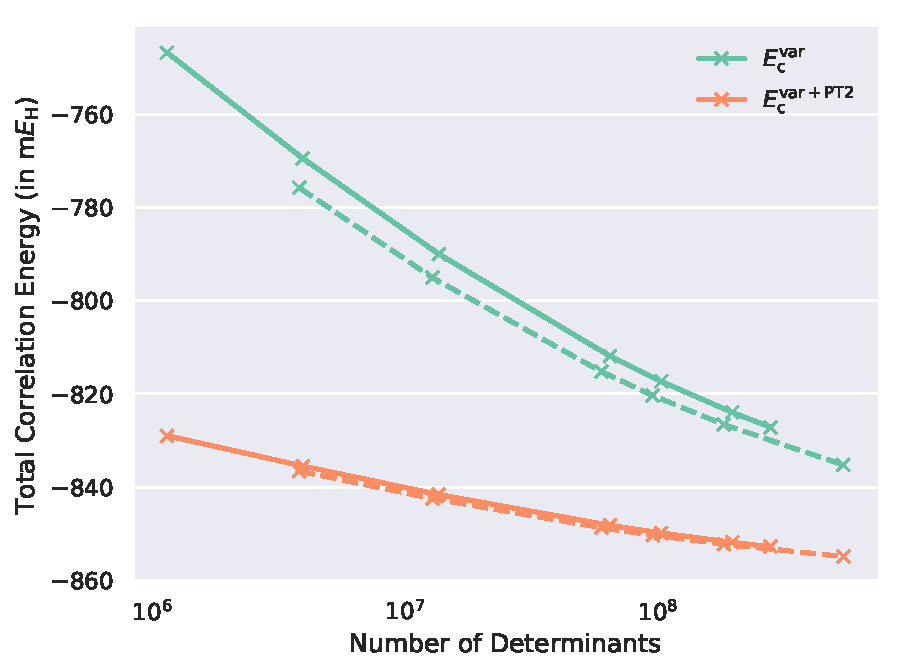
\includegraphics[scale=0.75]{figures/shci/shci.pdf}
%\caption{SHCI results. Original results are plotted with solid lines, updated localized orbital results (not part of main study) are plotted with dashed lines.}
\caption{SHCI energies versus number of determinants.  Blind test energies are plotted with solid lines, updated energies obtained with further optimized orbitals (not part of main study) are plotted with dashed lines.}
\label{shci_SI_fig}
\end{center}
\vspace{-0.6cm}
\end{figure}
%
The final energy is obtained by a weighted fit of the total energies to a quadratic function of the perturbative correction, as shown in Fig.~\ref{fig:shci_energy_blind} for the calculation submitted for the blind test, and in Fig.~\ref{fig:shci_energy_later} for the subsequent calculation that used better optimized orbitals and smaller values of $\epsilon_1$. The weight function used is the inverse square of the perturbative correction. Table~\ref{shci_energies} shows the same information in greater detail, including also the values of $\epsilon_1$ used
and the number of time-reversal symmetrized determinants and the number of determinants. Our largest calculation included $\num{5.4e8}$ determinants.\\

%
\begin{table}[ht!]
\begin{center}
\caption{SHCI variational and total energy convergence.  The top block of the table is for the
partially optimized orbitals used in the blind test, whereas the bottom block is for further optimized orbitals
and a smaller values of $\epsilon_1$.  The errors in the total energies, $E_{\rm tot}$, for finite values of $\epsilon_1$ are
statistical errors.  These are negligible, particularly for the smaller $\epsilon_1$ values.
The errors in $E_{\rm tot}$ extrapolated to $\epsilon_1=0$ are fit errors
which typically greatly underestimate the actual extrapolation error.  The energy reported in the blind test was that from the
7-point fit, with a conservative estimate of the extrapolation error which is almost an order of magnitude larger
than the fit error.}
\label{shci_energies}
\begin{tabular}{rrrll}
\toprule
%\multicolumn{1}{c|}{Method} & \multicolumn{1}{c}{$\Delta E$/m$E_{\text{H}}$} \\
\multicolumn{1}{c}{$\epsilon_1$} & \multicolumn{1}{c}{$N^{\rm sym}_{\rm det}$} & \multicolumn{1}{c}{$N_{\rm det}$} & \multicolumn{1}{c}{$E_{\rm var}$} & \multicolumn{1}{c}{$E_{\rm tot}$} \\
\midrule
$2.0 \times 10^{-4}$ &      579\,708 &   1\,134\,081 & $-231.468\,564$   & $-231.550\,787$ $\pm$ 0.000\,010 \\
$1.0 \times 10^{-4}$ &   1\,975\,676 &   3\,901\,848 & $-231.491\,252$   & $-231.557\,309$ $\pm$ 0.000\,010 \\
$5.0 \times 10^{-5}$ &   6\,790\,526 &  13\,486\,304 & $-231.511\,826$   & $-231.563\,444$ $\pm$ 0.000\,007 \\
$2.0 \times 10^{-5}$ &  32\,178\,640 &  64\,100\,382 & $-231.533\,720$   & $-231.570\,044$ $\pm$ 0.000\,005 \\
$1.5 \times 10^{-5}$ &  51\,218\,692 & 102\,088\,555 & $-231.539\,142$   & $-231.571\,697$ $\pm$ 0.000\,005 \\
$1.0 \times 10^{-5}$ &  97\,754\,454 & 194\,977\,798 & $-231.545\,790$   & $-231.573\,686$ $\pm$ 0.000\,003 \\
$8.0 \times 10^{-6}$ & 138\,641\,259 & 276\,617\,654 & $-231.548\,984$   & $-231.574\,641$ $\pm$ 0.000\,003 \\
Extrap. using 7 pts. &&&                               $-231.586\,064$   & $-231.586\,064$ $\pm$ 0.000\,160 \\
Extrap. using 6 pts. &&&                               $-231.585\,772$   & $-231.585\,772$ $\pm$ 0.000\,120 \\
Extrap. using 5 pts. &&&                               $-231.585\,569$   & $-231.585\,569$ $\pm$ 0.000\,143 \\
\midrule
$1.0 \times 10^{-4}$ &   1\,914\,692 &   3\,780\,337 & $-231.497\,568$   & $-231.558\,399$ $\pm$ 0.000\,010 \\
$5.0 \times 10^{-5}$ &   6\,410\,037 &  12\,722\,141 & $-231.516\,872$   & $-231.564\,290$ $\pm$ 0.000\,006 \\
$2.0 \times 10^{-5}$ &  29\,787\,396 &  59\,310\,339 & $-231.537\,074$   & $-231.570\,545$ $\pm$ 0.000\,006 \\
$1.5 \times 10^{-5}$ &  47\,463\,030 &  94\,569\,745 & $-231.542\,155$   & $-231.572\,140$ $\pm$ 0.000\,006 \\
$1.0 \times 10^{-5}$ &  90\,601\,302 & 180\,662\,587 & $-231.548\,415$   & $-231.574\,081$ $\pm$ 0.000\,002 \\
$5.0 \times 10^{-6}$ & 268\,931\,930 & 536\,792\,289 & $-231.557\,059$   & $-231.576\,736$ $\pm$ 0.000\,002 \\
Extrap. using 6 pts. &&&                               $-231.585\,609$   & $-231.585\,609$ $\pm$ 0.000\,104 \\
Extrap. using 5 pts. &&&                               $-231.585\,464$   & $-231.585\,464$ $\pm$ 0.000\,105 \\
\midrule
\end{tabular}
\end{center}
\end{table}
%
The total energy provided for the blind test, $-231.5861$ $E_{\text{H}}$ was the value from the 7-point weighted quadratic fit shown in Table~\ref{shci_energies} along with a conservative estimate for the extrapolation error of $1.5$ m$E_{\text{H}}$, which is almost an order of magnitude larger than the fit error. This corresponds to a correlation energy of $-864.2$ m$E_{\text{H}}$. In contrast to the statistical error, which has a well-defined probabilistic meaning, there is no well defined method for estimating the extrapolation error and different groups report wildly different estimates even when the underlying calculations are similar. In light of our subsequent calculations using better optimized orbitals and going down to smaller values of $\epsilon_1$, we could have gotten a slightly more accurate energy estimate of $-231.5856$ $E_{\text{H}}$ using the 5-point fit. Although the extrapolation curve is nearly linear, when sufficiently many data points are available, it is appropriate to perform a fit with a higher-order polynomial. The reduced chi-squared statistic can be used to avoid overfitting. A weighted cubic fit of either data set, using all the data points for that set, gives a total energy of $-231.5851$ $E_{\text{H}}$, corresponding to a correlation energy of
$-863.3$ m$E_{\text{H}}$. This should be considered to be the best post blind test SHCI estimate. Note that all the extrapolation estimates in this paragraph are well within the estimated error provided with the blind test.\\

All calculations were performed using the {\texttt{Arrow}} code~\cite{arrow}. For the blind test runs, the calculations shown in Table~\ref{shci_energies} for $\epsilon_1 = \num{2.e-4},\; \num{1.e-4},\; \num{5.e-5}$ and $\num{2.e-5}$ took in total 13 hours on four Intel(R) Xeon(R) Silver-4110 nodes (16 cores $@$ 2.1 GHz, 24 GB/core), and the calculations for $\epsilon_1 = \num{1.e-5}$ and $\num{8.e-6}$ took in total 49 hours on one Intel Xeon E7-8870v4 node (40 cores $@$ 2.1 GHz, 75 GB/core).

\begin{figure}[ht!]
\begin{center}
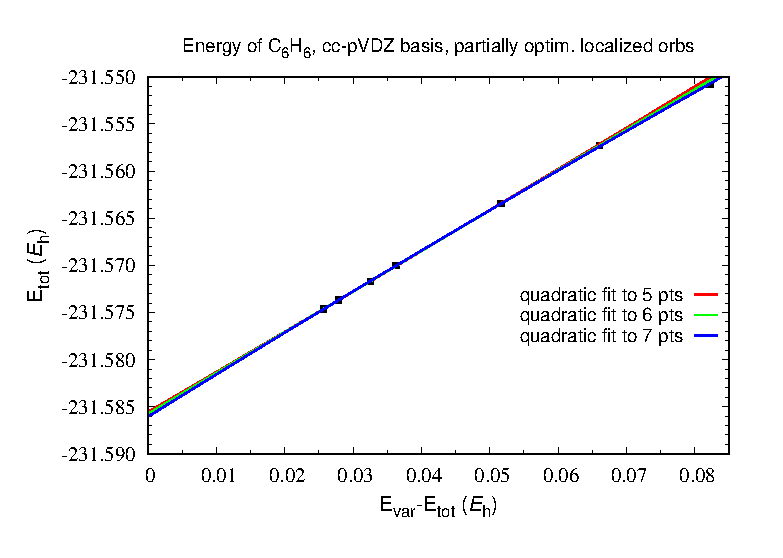
\includegraphics[scale=1.0]{figures/shci/energy_conv_C6H6_3a.eps}
\caption{Convergence plot of SHCI total energies for the partially optimized orbitals used in the blind test.
The lines are weighted quadratic fits, using varying number of points with the smallest $E_{\rm var}-E_{\rm tot}$ values.}
\label{fig:shci_energy_blind}
\end{center}
\end{figure}

\begin{figure}[ht!]
\begin{center}
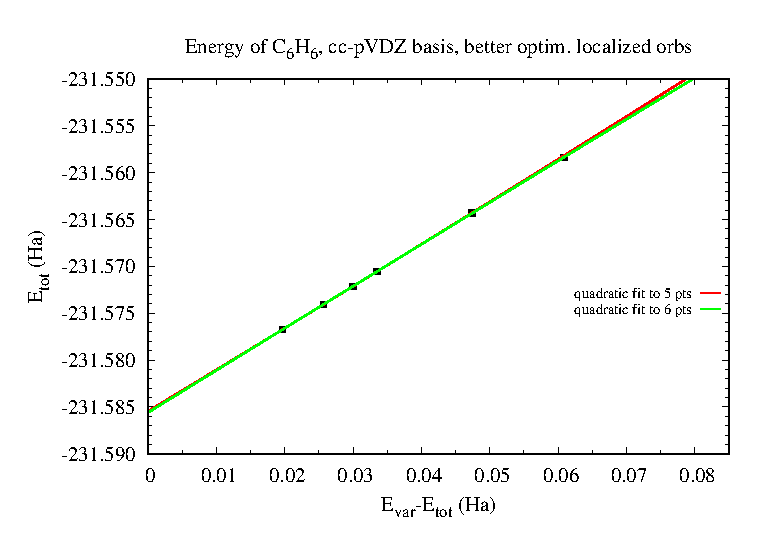
\includegraphics[scale=1.0]{figures/shci/energy_conv_C6H6_3b.eps}
\caption{Convergence plot of SHCI total energies for further optimized orbitals and smaller $\epsilon_1$ values.
The lines are weighted quadratic fits, using varying number of points with the smallest $E_{\rm var}-E_{\rm tot}$ values.}
\label{fig:shci_energy_later}
\end{center}
\end{figure}

\clearpage


\section{ASCI}
\label{sec:asci}
%
\begin{figure}[ht!]
\begin{center}
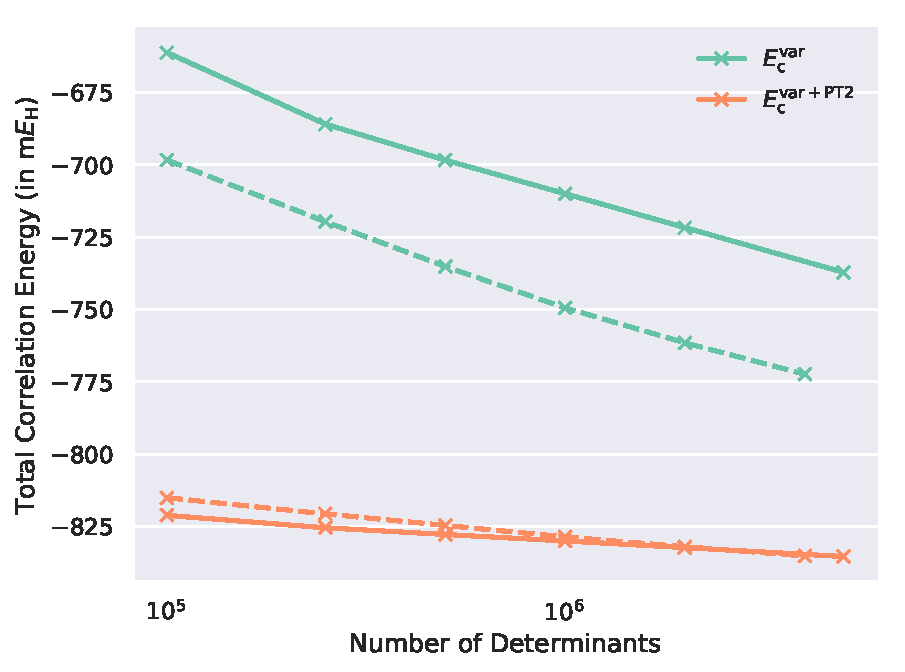
\includegraphics[scale=0.75]{figures/asci/asci.pdf}
\caption{ASCI results. Original results are plotted with solid lines, updated localized orbital results (not part of main study) are plotted with dashed lines.}
\label{asci_SI_fig}
\end{center}
\vspace{-0.6cm}
\end{figure}
%
Details on the most recent version of ASCI theory has recently been presented elsewhere~\cite{tubman_whaley_selected_ci_jctc_2020,tubman_whaley_selected_ci_pt_arxiv_2018}. 
All ASCI calculations were performed using a development version of Q-Chem 5.2\cite{shao2015advances}  on AMD EPYC 7401 hardware (2.0 GHz, 5.3 GB/core). The CI component was run in parallel over 24 processors but the subsequent Epstein-Nesbet PT2 correction was computed on a single processor. The active space orbitals were optimized from canonical HF MOs in an multiconfigurational self-consistent field (MCSCF) manner (while only considering active-active rotations, i.e. keeping the core levels frozen), using $5\times 10^5$ ASCI selected determinants  \cite{levine2020casscf}, prior to PT2 calculations with varying number of determinants. The computed ASCI results are presented in  Figure \ref{asci_SI_fig}, and the final extrapolated correlation energy is estimated to be $\Delta$E$_\textrm{ASCI}$ =-860.0 $\pm$ 0.2 m$E_{\text{H}}$ with the error bar spanned by the uncertainty in the extrapolation towards the limit of zero PT2 correction (standard deviation of a linear fit with last 3 points, as described in Ref \citenum{hait2019levels}).

\subsection{ASCI with localized orbitals}\label{sec:asciloc}

Subsequent to the blind challenge, an additional effort was made to determine the impact of using spatial symmetry broken localized orbitals as an initial guess instead of delocalized canonical MOs. The occupied canonical orbitals were consequently Pipek-Mezey localized\cite{pipek_mezey_jcp_1989} and the virtual space subjected to the Sano procedure\cite{sano2000elementary} to obtain the corresponding antibonding orbitals. These resulting orbitals were similarly optimized by active-active rotations in an MCSCF manner, using $5\times 10^5$ ASCI determinants\cite{levine2020casscf}. The optimized localized orbitals yielded significantly lower variational energies for a given size of ASCI wave function, although inclusion of PT2 resulted in values quite similar with those obtained from delocalized orbitals (as can be seen from Table \ref{tab:ascidata} and  Figure \ref{asci_SI_fig}). The lower magnitude of PT2 corrections nonetheless suggest that the localized orbital ASCI values are more reliable, especially with respect to extrapolation (by virtue of being closer to the $E_{PT2}\to 0$ limit). Extrapolation of the results obtained using localized orbitals to $E_{PT2}\to 0$ limit yields a correlation energy of $-861.3\pm0.5$ m$E_{\text{H}}$.\\

It is however worth noting that this localized orbital result is essentially outside the range estimated from the original delocalized case (-860.0 $\pm$ 0.2 m$E_{\text{H}}$). This, in conjunction with the relatively low magnitude of correlation energy predicted by ASCI relative to other methods, indicates that the extrapolated ASCI error bar estimate is much too small in this case. This is likely a consequence of the stubbornly large $E_{PT2}$ values for the variational subspace sizes considered (as can be seen from Table \ref{tab:ascidata}), which likely prevents attainment of the asymptotic $E_{PT2}\to 0$ regime behavior for the extrapolation (despite $r^2$ of the linear fit being very close to 1, which is the origin of the too small error bars). It is however also worth noting that the extrapolation protocol nonetheless is quite effective, recovering $\sim$ $-25/-26$ m$E_{\text{H}}$ of the $\sim$ $-28$ m$E_{\text{H}}$ correlation not recovered by ASCI+PT2 alone (assuming an actual correlation energy of $\sim$ $-863$ m$E_{\text{H}}$). More reliable estimates from ASCI+PT2 would require larger variational subspaces than those studied in this work. Our original choice was partly determined by code limitations, though we considered $5\times 10^6$ determinants to be sufficient at the time of the blind challenge. 
%
\begin{table}[]
	\begin{tabular}{llll|llll}
		\toprule
		\multicolumn{4}{l}{Delocalized Orbitals (original blind test)} & \multicolumn{4}{l}{Localized orbitals}             \\\hline
		$N_\text{dets}$      & $E_{\mathrm{c}}^{\mathrm{var}}$    & $E_{\mathrm{c}}^{\mathrm{PT2}}$      & $E_{\mathrm{c}}^{\mathrm{var+PT2}}$    & $N_\text{dets}$    & $E_{\mathrm{c}}^{\mathrm{var}}$ & $E_{\mathrm{c}}^{\mathrm{PT2}}$   & $E_{\mathrm{c}}^{\mathrm{var+PT2}}$ \\
		\midrule\midrule
		$1\times10^5$  & $-661.17$        & $-159.97$    & $-821.14$            & $1\times10^5$ & $-698.31$     & $-116.74$ & $-815.05$         \\
		$2.5\times10^5$    & $-685.91$        & $-139.54$    & $-825.45$            & $2.5\times10^5$ & $-719.63$     & $-101.03$ & $-820.65$         \\
		$5\times10^5$    & $-698.34$        & $-129.41$    & $-827.75$            & $5\times10^5$ & $-735.12$     & $-89.49$  & $-824.62$         \\
		$1\times10^6$    & $-709.96$        & $-120.04$    & $-830.00$            & $1\times10^6$ & $-749.43$     & $-79.17$  & $-828.60$         \\
		$2\times10^6$    & $-721.68$        & $-110.61$    & $-832.29$            & $2\times10^6$ & $-761.51$     & $-70.49$  & $-832.00$         \\
		$5\times10^5$    & $-737.13$        & $-98.25$     & $-835.38$            & $4\times10^5$ & $-772.35$     & $-62.83$  & $-835.18$         \\\hline 
		Fit         &                &            & $-860.0\pm0.2$            & Fit      &             &         & $-861.3\pm0.5$ \\
		\midrule
	\end{tabular}
	\caption{Correlation energies  ($E_{\mathrm{c}}$, in m$E_{\text{H}}$) for ASCI wave functions with various number of determinants ($N_\text{dets}$).}
	\label{tab:ascidata}
	\vspace{-0.6cm}
\end{table}

\section{iCI}

The iCI approach~\cite{liu_hoffmann_ici_jctc_2016,liu_hoffmann_ici_jctc_2020}, which was born from the restricted static-dynamic-static~\cite{liu_hoffmann_sds_tca_2014} (SDS) framework for treating strongly correlated electrons, is a method designed to converge from above to the FCI limit within just a few iterations, by constructing and diagonalizing a $3N_P\times3N_P$ Hamiltonian matrix at each macro/micro-iteration, even when starting with a very poor initial guess. Here, $N_P$ denotes the number of target states. This convergence behaviour is hardly surprising, since the lowest order realization of the SDS framework, i.e., SDSPT2~\cite{liu_hoffmann_sdspt2_mp_2017}, already performs very well for prototypical systems of variable near degeneracies. However, iCI is computationally very expensive. One way out is to combine iCI with the idea of configuration selection, so as to generate a compact variational space for static correlation. The remaining dynamic correlation is treated via Epstein-Nesbet PT2. In brief, iCI has the following features: {\bf{(i)}} Full spin symmetry is always maintained by taking configuration state functions (CSF) as the many-electron basis. {\bf{(ii)}} Although the selection is performed on individual CSFs, it is orbital configurations (oCFG) that are used as the organizing units. {\bf{(iii)}} Given a coefficient pruning threshold, $C_{\text{min}}$ (which determines the size of the variational space for static correlation), the selection of important oCFGs/CSFs is performed iteratively until convergence. {\bf{(iv)}} At each iteration in the growth of the wave function, the first-order interacting space is decomposed into disjoint subspaces, so as to reduce memory requirement on one hand and facilitate parallelization on the other. {\bf{(v)}} Upper bounds (which involve only two-electron integrals) for the interactions between doubly connected oCFG pairs are used to screen each first-order interacting subspace before the first-order coefficients of individual CSFs are evaluated. {\bf{(vi)}} The diagonalization of the Hamiltonian matrix in the variational space is achieved by the iterative vector interaction (iVI) method\cite{iVIa,iVIb} (which, for $N_p$ roots, constructs and diagonalizes a $3N_p\times 3N_p$ matrix in each iteration). {\bf{(vii)}} Upon termination of the selection, dynamic correlation is estimated by using state-specific Epstein-Nesbet PT2 (iCIPT2). Results were obtained in $D_{2\text{h}}$ point group symmetry using either HF or natural (NO) orbitals, cf. Fig. \ref{ici_SI_fig}, of which the linearly extrapolated (using the last six data points) iCIPT2(NO) result of $\Delta E_{\text{iCIPT2(NO)}} = -861.05\pm0.5$ m$E_{\text{H}}$ is used in Fig. 1 of the main study, cf. Table \ref{OldNO} and Fig. \ref{BenzeneEn}. Calculations were run using BDF (Beijing Density Functional) program~\cite{bdf_prog_tca_1997,bdf_prog_jcp_2020} on a single node with two Intel Xeon E5-2640 v3 processors (16 cores $@$ 2.6 GHz, 8.0 GB/core), and the OpenMP efficiency was approximately $50$ $\%$.\\

%
\begin{figure}[ht!]
\begin{center}
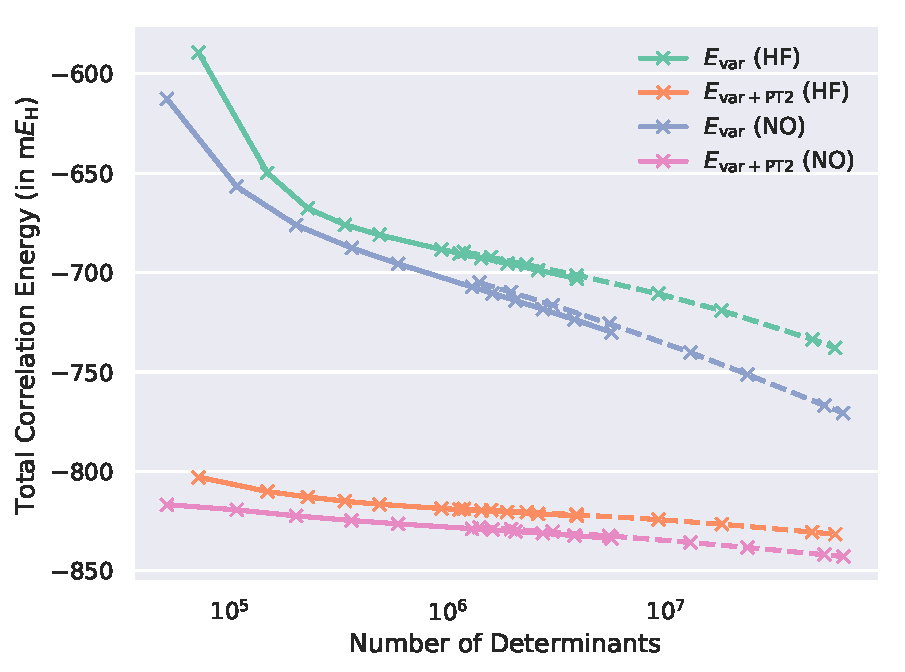
\includegraphics[scale=0.75]{figures/ici/ici.pdf}
\caption{iCI results. Original results are plotted with solid lines, updated results (not part of main study) are plotted with dashed lines.}
\label{ici_SI_fig}
\end{center}
\vspace{-0.6cm}
\end{figure}
%
Following the submission of the iCI result in Fig. 1 of the main study (Ref. \citenum{liu_hoffmann_ici_jctc_2020}), the efficiency of the method was increased by a factor of nearly 20. As such, the same $C_{\text{min}}$ values now always lead to smaller variational space, which has allowed for larger calculations than what was previously possible using either canonical HF orbitals or NOs. These updated results (not part of the blind challenge) are also presented in Fig. \ref{ici_SI_fig} (with dashed lines), cf. also Table \ref{NewNO} and Fig. \ref{BenzeneEnNew}. These are estimated to be more accurate than the original results since the selected variational space is larger. Moreover, the updated iCIPT2(NO) results are again estimated to be more reliable than the corresponding iCIPT2(HF) results since the former are always lower than the latter for each considered $C_{\text{min}}$ value. Furthermore, the gap between the smallest $C_{\text{min}}$ value and the extrapolated value is smaller for iCIPT2(NO) than for iCIPT2(HF). The linear extrapolations (again not shown) yield final correlation energies of $\Delta E_{\text{iCIPT2(HF,new)}} = -866.07\pm1.0$ m$E_{\text{H}}$ and $\Delta E_{\text{iCIPT2(NO,new)}} = -864.15\pm0.6$ m$E_{\text{H}}$.\\

For both the original and the updated results, the remaining difference between HF- and NO-based iCIPT2 (ca. 2 m$E_{\text{H}}$) may be understood in terms of space dimensions, as the cumulative effect of the unsampled CSFs remains substantial. To verify this argument, Cr$_2$/AVDZ may be used as an example. The difference between iCIPT2(HF) and iCIPT2(NO) in this case is within $0.1$ m$E_{\text{H}}$, correlating with the fact that the sampled space of CSFs makes up a considerably larger part of the FCI Hilbert space.

\begin{table}[!htp]
	\small
\caption{iCIPT2 blind-test correlation energies for benzene with natural orbitals }
	\begin{threeparttable}
		\centering
	\begin{tabular}{c|rrrrrrr}\toprule
		C$_{\text{min}}$&$N_{\mathrm{cfg}}$&$\tilde{N}_{\mathrm{csf}}$\tnote{a}&$\tilde{N}_{\mathrm{det}}$\tnote{b}
%		&$N_{csf,Q}$\tnote{c}
		&$E_{\mathrm{c}}^{\mathrm{var}}/\mathrm{mE_h}$&$E_{\mathrm{c}}^{\mathrm{PT2}}/\mathrm{mE_h}$&$E_{\mathrm{c}}/\mathrm{mE_h}$&$T/s$\tnote{c}\\\toprule
			$1.0\times10^{-3}$ &    14496 &    17890 &  50944&  $-612.591$  &  $-204.133$&  $-816.724$ &379\\
			$5.0\times10^{-4}$ &    28188 &    36448 & 106317&  $-656.729$  &  $-162.637$&  $-819.366$ &669\\
			$3.0\times10^{-4}$ &    48373 &    65080 & 199486&  $-676.147$  &  $-146.237$&  $-822.384$ &1481\\
			$2.0\times10^{-4}$ &    78947 &   109831 & 358274&  $-687.627$  &  $-137.072$&  $-824.699$ &2794\\
			$1.5\times10^{-4}$ &   119580 &   170356 & 586272&  $-695.623$  &  $-130.780$&  $-826.403$ &5066\\
			$1.0\times10^{-4}$ &   234640 &   344959 &1277001&  $-707.243$  &  $-121.564$&  $-828.807$ &15206\\
			$9.0\times10^{-5}$ &   284068 &   421316 &1585683&  $-710.440$  &  $-119.020$&  $-829.460$ &22335\\
			$8.0\times10^{-5}$ &   353743 &   529909 &2028558&  $-714.110$  &  $-116.113$&  $-830.223$ &38399\\
			$7.0\times10^{-5}$ &   456337 &   692215 &2697171&  $-718.441$  &  $-112.694$&  $-831.135$ &49238\\
			$6.0\times10^{-5}$ &   615593 &   947846 &3759324&  $-723.616$  &  $-108.673$&  $-832.289$ &77344\\
			$5.0\times10^{-5}$ &   878837 &  1381837 &5580152&  $-729.983$  &  $-103.707$&  $-833.690$ &133551\\\midrule
			0.0\tnote{b}&&&&&&\multicolumn{2}{c}{$-861.05\pm0.51$}\\\bottomrule
		\end{tabular}
\begin{tablenotes}
\item[a]Number of selected CSFs.
\item[b]Estimated number of determinants according to the expression $\sum_I\frac{\tilde{N}_{\mathrm{csf}}^I}{N_{\mathrm{csf}}^I}N_{\mathrm{det}}^I$, with $N_{\mathrm{det}}^I$, $N_{\mathrm{csf}}^I$ and $\tilde{N}_{\mathrm{csf}}^I$ being the numbers of determinants, CSFs and selected CSFs of orbital configuration (oCFG) $I$, respectively.
\item[c](1) CPU: Intel(R) Xeon(R) E5--2640 v3$\times$2, 16 cores; (2) memory: 128 Gb;
			(3) parallelization: OpenMP, 16 threads.
\item[d]Linearly extrapolated result using values of the 9 smallest $C_{min}$. The error bar refers to the half length of 95\% confidence interval.
		\end{tablenotes}
	\end{threeparttable}
	\label{OldNO}
\end{table}

\begin{table}[!htp]
	\small
	\caption{iCIPT2 blind-test correlation energies for benzene with Hartree-Fock orbitals }
	\begin{threeparttable}
		\centering
	\begin{tabular}{c|rrrrrrr}\toprule
		C$_{\text{min}}$&$N_{\mathrm{cfg}}$&$\tilde{N}_{\mathrm{csf}}$\tnote{a}&$\tilde{N}_{\mathrm{det}}$\tnote{b}
%		&$N_{csf,Q}$\tnote{c}
		&$E_{\mathrm{c}}^{\mathrm{var}}/\mathrm{mE_h}$&$E_{\mathrm{c}}^{\mathrm{PT2}}/\mathrm{mE_h}$&$E_{\mathrm{c}}/\mathrm{mE_h}$&$T/s$\tnote{c}\\\toprule
			$1.0\times10^{-3}$ &    19811 &    24862 &  71137&  $-589.336$  &  $-213.573$&  $-802.909$ &301  \\
			$5.0\times10^{-4}$ &    38400 &    51025 & 147228&  $-649.922$  &  $-160.205$&  $-810.127$ &837  \\
			$3.0\times10^{-4}$ &    54907 &    76712 & 225685&  $-667.714$  &  $-145.170$&  $-812.884$ &1309 \\
			$2.0\times10^{-4}$ &    75868 &   109263 & 333495&  $-675.959$  &  $-139.038$&  $-814.997$ &2363 \\
			$1.5\times10^{-4}$ &   103807 &   150972 & 480806&  $-681.083$  &  $-135.481$&  $-816.564$ &3036 \\
			$1.0\times10^{-4}$ &   180981 &   269149 & 921928&  $-688.358$  &  $-130.306$&  $-818.664$ &9875 \\
			$9.0\times10^{-5}$ &   214438 &   320658 &1120558&  $-690.363$  &  $-128.831$&  $-819.194$ &12712\\
			$8.0\times10^{-5}$ &   261828 &   394778 &1410356&  $-692.695$  &  $-127.102$&  $-819.797$ &17447\\
			$7.0\times10^{-5}$ &   331831 &   505250 &1849734&  $-695.422$  &  $-125.065$&  $-820.487$ &26334\\
			$6.0\times10^{-5}$ &   444010 &   683971 &2570589&  $-698.767$  &  $-122.563$&  $-821.330$ &42053\\
			$5.0\times10^{-5}$ &   640800 &  1001148 &3869123&  $-703.066$  &  $-119.361$&  $-822.427$ &72945\\\midrule
			0.0\tnote{b}&&&&&&\multicolumn{2}{c}{$-863.32\pm0.54$}\\\bottomrule
		\end{tabular}
\begin{tablenotes}
\item[a]Number of selected CSFs.
\item[b]Estimated number of determinants according to the expression $\sum_I\frac{\tilde{N}_{\mathrm{csf}}^I}{N_{\mathrm{csf}}^I}N_{\mathrm{det}}^I$, with $N_{\mathrm{det}}^I$, $N_{\mathrm{csf}}^I$ and $\tilde{N}_{\mathrm{csf}}^I$ being the numbers of determinants, CSFs and selected CSFs of orbital configuration (oCFG) $I$, respectively.
\item[c](1) CPU: Intel(R) Xeon(R) E5--2640 v3$\times$2, 16 cores; (2) memory: 128 Gb;
			(3) parallelization: OpenMP, 16 threads.
\item[d]Linearly extrapolated result using values of the 6 smallest $C_{min}$. The error bar refers to the half length of 95\% confidence interval.
		\end{tablenotes}
	\end{threeparttable}
	\label{OldHF}
\end{table}

\begin{figure}[!htp]
	\centering
	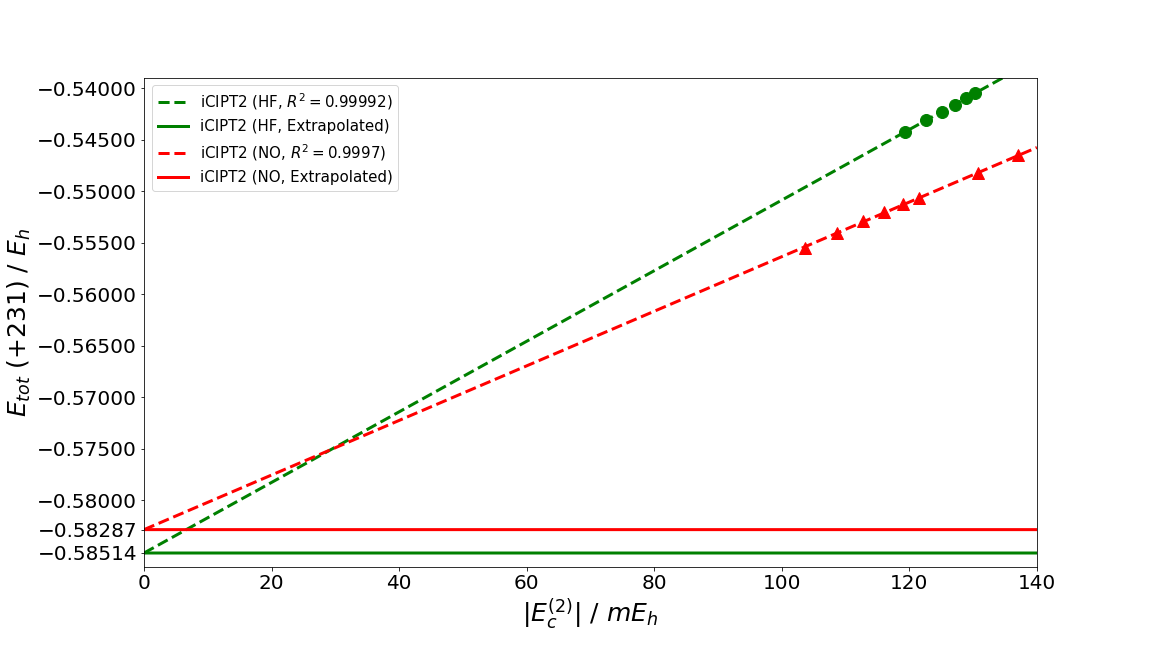
\includegraphics[width=\textwidth]{figures/ici/benzene_ici.png}
	\caption{ Linear fit of the correlation energy of benzene (blind test).}\label{BenzeneEn}
\end{figure}

\begin{table}[!htp]
	\small
	\caption{iCIPT2 correlation energies for benzene with natural orbitals (updated results).}
\begin{threeparttable}
	\centering
	\begin{tabular}{c|rrrrrrr}\toprule
		C$_{\text{min}}$&$N_{\mathrm{cfg}}$&$\tilde{N}_{\mathrm{csf}}$\tnote{a}&$\tilde{N}_{\mathrm{det}}$\tnote{b}
%		&$N_{csf,Q}$\tnote{c}
		&$E_{\mathrm{c}}^{\mathrm{var}}/\mathrm{mE_h}$&$E_{\mathrm{c}}^{\mathrm{PT2}}/\mathrm{mE_h}$&$E_{\mathrm{c}}/\mathrm{mE_h}$&$T/s$\tnote{c}\\\toprule
		$6.0\times10^{-5}$ &   245224 &   379662 & 1379097
%		& 2.74$\times10^{11}$
		&  $-705.099$  &  $-122.996$&  $-828.095$ &491\\
		$5.0\times10^{-5}$ &   330089 &   518448 & 1932040
%		& 4.00$\times10^{11}$
		&  $-709.899$  &  $-119.182$&  $-829.081$ &670\\
		$4.0\times10^{-5}$ &   486177 &   778940 & 2991370
%		& 6.42$\times10^{11}$
		&  $-716.354$  &  $-114.087$&  $-830.441$ &1039\\
		$3.0\times10^{-5}$ &   830917 &  1369463 & 5436028
%		& 1.17$\times10^{12}$
		&  $-725.650$  &  $-106.817$&  $-832.467$ &1834\\
		$2.0\times10^{-5}$ &  1809463 &  3121693 &12849733
%		& 2.65$\times10^{12}$
		&  $-740.245$  &  $-95.513$&  $-835.758$ &4273\\
		$1.5\times10^{-5}$ &  3134922 &  5595481 &23479710
%		& 4.52$\times10^{12}$
		&  $-751.271$  &  $-87.026$&  $-838.298$ &7597\\
		$1.0\times10^{-5}$ &  6555147 & 12315752 &52744912
%		& 8.88$\times10^{12}$
		&  $-766.783$  &  $-75.134$&  $-841.918$ &19299\\
		$9.0\times10^{-6}$ &  7869797 & 14995161 &64497488
%		& 1.04$\times10^{13}$
		&  $-770.695$  &  $-72.139$&  $-842.834$ &33344\\\midrule
		0.0\tnote{d}&&&&&&\multicolumn{2}{c}{$-864.15\pm0.57$}\\\bottomrule
	\end{tabular}
\begin{tablenotes}
	\item[a]Number of selected CSFs.
	\item[b]Estimated number of determinants according to the expression $\sum_I\frac{\tilde{N}_{\mathrm{csf}}^I}{N_{\mathrm{csf}}^I}N_{\mathrm{det}}^I$, with $N_{\mathrm{det}}^I$, $N_{\mathrm{csf}}^I$ and $\tilde{N}_{\mathrm{csf}}^I$ being the numbers of determinants, CSFs and selected CSFs of orbital configuration (oCFG) $I$, respectively.
%	\item[c]Number of CSFs in Q space.
	\item[c](1) CPU: Intel(R) Xeon(R) Gold 6240 $\times$4, 72 cores; (2) memory: 768 Gb; (3) parallelization: OpenMP, 72 threads.
	\item[d]Linearly extrapolated result using values of the 6 smallest $C_{min}$. The error bar refers to the half length of 95\% confidence interval.
\end{tablenotes}
\end{threeparttable}
\label{NewNO}
\end{table}

\begin{table}[!htp]
	\small
	\caption{iCIPT2 correlation energies for benzene with Hartree-Fock orbitals (updated results).}
\begin{threeparttable}
	\begin{tabular}{c|rrrrrrr}\toprule
		C$_{\text{min}}$&$N_{\mathrm{cfg}}$&$\tilde{N}_{\mathrm{csf}}$\tnote{a}&$\tilde{N}_{\mathrm{det}}$\tnote{b}
%		&$N_{csf,Q}$\tnote{c}
		&$E_{\mathrm{c}}^{\mathrm{var}}/\mathrm{mE_h}$&$E_{\mathrm{c}}^{\mathrm{PT2}}/\mathrm{mE_h}$&$E_{\mathrm{c}}/\mathrm{mE_h}$&$T/s$\tnote{c}\\\toprule
	$6.0\times10^{-5}$ &  221314 &   338334 & 1172202
%	&  1.76$\times10^{11}$
	& $-689.523$ &    $-129.322$ &  $-818.846$ &326\\
	$5.0\times10^{-5}$ &  282405 &   439038 & 1561473
%	&  2.38$\times10^{11}$
	& $-692.337$ &    $-127.201$ &  $-819.539$ &426\\
	$4.0\times10^{-5}$ &  391414 &   620645 & 2273564
%	&  3.63$\times10^{11}$
	& $-696.048$ &    $-124.424$ &  $-820.473$ &621\\
	$3.0\times10^{-5}$ &  631646 &  1017094 & 3856238
%	&  6.86$\times10^{11}$
	& $-701.315$ &    $-120.475$ &  $-821.790$ &1109\\
	$2.0\times10^{-5}$ & 1398298 &  2301712 & 9150757
%	&  1.86$\times10^{12}$
	& $-710.687$ &    $-113.578$ &  $-824.265$ &2749\\
	$1.5\times10^{-5}$ & 2583842 &  4359388 &17861976
%	&  3.66$\times10^{12}$
	& $-719.137$ &    $-107.437$ &  $-826.574$ &5387\\
	$1.0\times10^{-5}$ & 6206395 & 10978445 &46457235
%	&  8.63$\times10^{12}$
	& $-733.630$ &    $-96.926$ &  $-830.557$ &14470\\
	$9.0\times10^{-6}$ & 7736950 & 13878500 &59119837
%	&  1.05$\times10^{13}$
	& $-737.772$ &    $-93.920$ &  $-831.692$ &20203\\\midrule
	0.0\tnote{b}&&&&&&\multicolumn{2}{c}{$-866.07\pm0.99$}\\\bottomrule
	\end{tabular}
\begin{tablenotes}
	\item[a]Number of selected CSFs.
	\item[b]Estimated number of determinants according to the expression $\sum_I\frac{\tilde{N}_{\mathrm{csf}}^I}{N_{\mathrm{csf}}^I}N_{\mathrm{det}}^I$, with $N_{\mathrm{det}}^I$, $N_{\mathrm{csf}}^I$ and $\tilde{N}_{\mathrm{csf}}^I$ being the numbers of determinants, CSFs and selected CSFs of orbital configuration (oCFG) $I$, respectively.
%	\item[c]Number of CSFs in Q space.
	\item[c](1) CPU: Intel(R) Xeon(R) Gold 6240 $\times$4, 72 cores; (2) memory: 768 Gb; (3) parallelization: OpenMP, 72 threads.
	\item[d]Linearly extrapolated result using values of the 6 smallest $C_{min}$. The error bar refers to the half length of 95\% confidence interval.
\end{tablenotes}
\end{threeparttable}
\label{NewHF}
\end{table}

\begin{figure}[!htp]
	\centering
	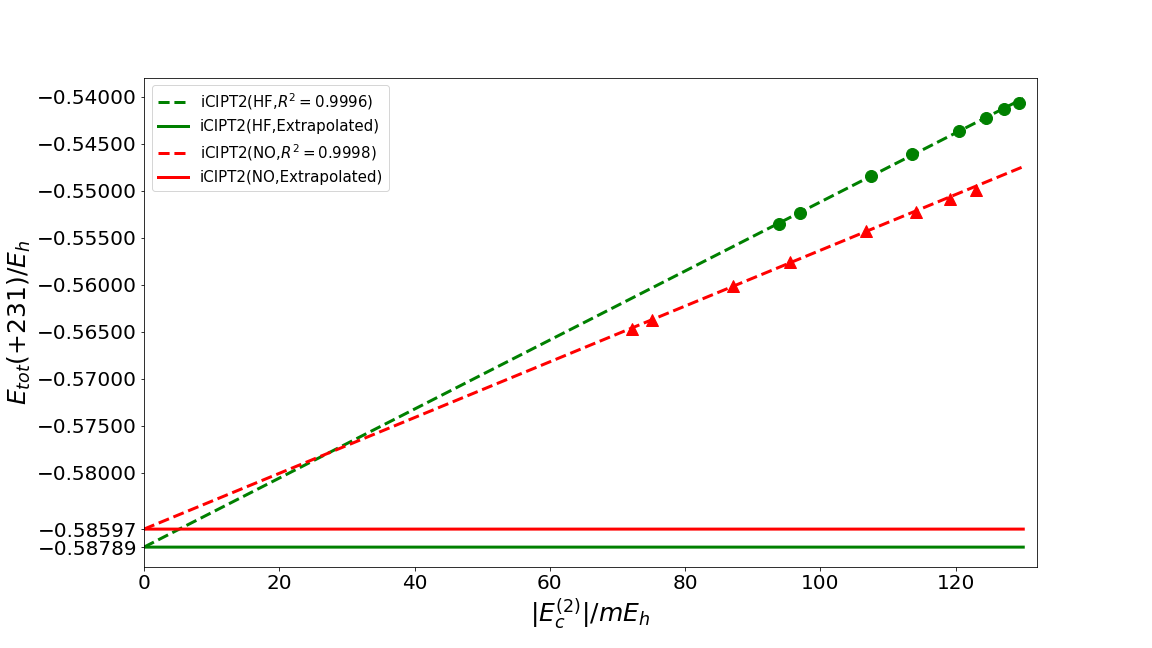
\includegraphics[width=\textwidth]{figures/ici/benzene_ici_updated.png}
	\caption{Linear fit of the correlation energy of benzene (updated results).}\label{BenzeneEnNew}
\end{figure}

\begin{table}[!htp]
	\centering
	\caption{Linearly extrapolated iCIPT2 correlation energies ($E_{\mathrm{c}}$ in $\mathrm{mE_h}$) for benzene and
extrapolation errors (in $\mathrm{mE_h}$). A: extrapolation distance; B: standard deviation; C:
half length of 95\% confidence interval.}
	\begin{tabular}{ccccccrc}\toprule
		&Orbitals
		&\makecell{$E_{\mathrm{c}}$}
		&\makecell{A}
		&\makecell{B}
		&\makecell{C}
		&CPU/h&memory/Gb
		\\\toprule
		\multirow{2}{*}{Blind Test}
		&NO&$-861.05$&27.36&0.22&0.51&1545&$\sim$650\\
		&HF&$-863.32$&40.89&0.19&0.54&836&$\sim$650\\\midrule
		\multirow{2}{*}{Updated}
		&NO&$-864.15$&21.32&0.21&0.57&1348&$\sim$610\\
		&HF&$-866.07$&34.38&0.36&0.99&891&$\sim$610\\\bottomrule
	\end{tabular}
\label{iCIsum}
\end{table}

\section{FCCR}

The size-extensive FCCR method exploits screenings within the single-reference CC formalism for constructing the excitation manifold $({\mathcal P})$ and to exclude insignificant operation mostly arising from the nonlinear terms of the working equation~\cite{ten_no_fcc_prl_2018}. The subsequent FCCR(2) computes the second-order perturbative correction to FCCR using the entire interacting space $({\mathcal Q})$ orthogonal to ${\mathcal P}$ generated through $[\hat H, \hat T_{\rm FCCR}]$~\cite{ten_no_fccr_2020}. For single-reference systems, FCCR(2') which approximate the $\hat \lambda$ amplitudes by $\hat T^{\dagger}$ is also available. All calculations were performed using the \texttt{GELLAN} program~\cite{gellan} in parallel on Intel Xeon Gold 6148 nodes (40 cores @ 2.4 GHz).\\

%
\begin{table}[ht!]
\begin{center}
\caption{FCCR calculation details (blind test).}
\label{fccr_SI_table}
\begin{tabular}{l|r}
\toprule
\multicolumn{1}{c|}{Method} & \multicolumn{1}{c}{$\Delta E$/m$E_{\text{H}}$} \\
\midrule\midrule
FCCR(MP) & $-860.1$ \\
FCCR(EN) & $-865.4$ \\
FCCR(avg) & $-862.8$ \\
FCCR(avg) + $\vartheta_{\mathcal O}$ corr. & $-863.0$ \\
\midrule
\end{tabular}
\vspace{-0.6cm}
\end{center}
\end{table}
%
Table \ref{fccr_SI_table} shows the result of FCCR(2') with the M{\o}ller-Plesset (MP) and Epstein-Nesbet (EN) partitionings with the connectivity threshold $\vartheta_{\mathcal C}=0.03$ and the operation threshold $\vartheta_{\mathcal O}=3.0 \times 10^{-7}$ as combined with the exclusion-principle-violating (EPV) form of the screening~\cite{ten_no_fcc_prl_2018}, leading to 4,818,644 FCCR cluster amplitudes. The FCI energy is estimated to lie very close to the average of the MP and EN results from various benchmarks (avg.), which may further be corrected for $\vartheta_{\mathcal O}$ based on CCSD, resulting in the estimate $-862.98 {\rm m}E_{\rm H}$. This calculation required 0.1M core hours invoking 640 MPI processes. The interacting space ${\mathcal Q}$ for the second-order correction is perfectly distributed to the processes, and the memory requirement of the present FCCR(2') calculation is at most 2GB per process.\\

%
\begin{table}[ht!]
\begin{center}
\caption{FCCR calculation details (updated results).}
\label{fccr_update_SI_table}
\begin{tabular}{r|r|r|r|r}
\toprule
\multicolumn{1}{c|}{$\vartheta_{\mathcal{P}}$} & \multicolumn{1}{c|}{$\Delta E$/m$E_{\text{H}}$} & \multicolumn{1}{c|}{$N_{\mathcal{P}}$} & \multicolumn{1}{c|}{$E^{(2)}$/m$E_{\text{H}}$} & \multicolumn{1}{c}{$N_{\mathcal{Q}}$} \\
\midrule\midrule
$5\times10^{-4}$   &  $-849.05$ & 109,860 & $-81.09$ & $2.2\times10^{8}$ \\
$4\times10^{-4}$   &  $-852.25$ & 137,421 & $-62.36$ & $2.6\times10^{8}$ \\
$3\times10^{-4}$   &  $-854.93$ & 174,914 & $-46.71$ & $3.7\times10^{8}$ \\
$2\times10^{-4}$   &  $-856.84$ & 229,842 & $-35.11$ & $6.4\times10^{8}$ \\
\hline
\multicolumn{1}{c|}{extrap.} &  $-862.83$ & \multicolumn{1}{c|}{---} & 0.0 & \multicolumn{1}{c|}{---} \\
\midrule
\end{tabular}
\vspace{-0.6cm}
\end{center}
\end{table}
%
A fast and more systematic estimate of the FCI limit is enabled by the extrapolation of FCCR(2). Table \ref{fccr_update_SI_table} presents an updated FCCR(2) correlation energy (not part of the blind challenge) along with the second-order correction of the MP partitioning as a function of the principal screening threshold $\vartheta\rm_{\mathcal P}$. Besides $\vartheta_{\mathcal O}$, the latest implementation of FCCR(2) controls the excitation manifold in terms of the two screening parameters, $\vartheta_{\mathcal P}$ to select the cluster operators of ${\mathcal P}$ perturbatively and $\vartheta_{\mathcal G}$ for the generator space $({\mathcal G})$ to discriminate strong correlation in ${\mathcal P}$.\cite{ten_no_fccr_2020} Except for $\vartheta_{\mathcal P}$, all screening parameters are fixed to be $\vartheta_{\mathcal G}=0.01$, $\vartheta_{\mathcal O}=10^{-7}$ for FCCR, and $\vartheta_{\mathcal O}=3.0\times10^{-6}$ for $E^{(2)}$. Tightening $\vartheta\rm_{\mathcal P}$ increases the accuracy of FCCR(2) according to the increasing dimensions of ${\mathcal P}$ and ${\mathcal Q}$. It is found that a linear relationship holds~\cite{ten_no_fccr_2020} between $\Delta E_{\rm FCCR(2)}$ and $E^{\rm (2)}$, as shown in Fig. \ref{fccr_updated_SI_fig}, and the best estimate of FCCR(2) based on the extrapolation is $-862.83$ m$E_{\text{H}}$. The calculations for the four values of $\vartheta\rm_{\mathcal P}$ in Table \ref{fccr_update_SI_table} required 0.035M, 0.048M, 0.073M and 0.134M core hours, respectively, using 640 MPI processes. The algorithmic details of the FCCR(2) implementation and other applications will be elaborated in a separate paper~\cite{ten_no_fccr_2020}.
%
\begin{figure}[ht!]
\begin{center}
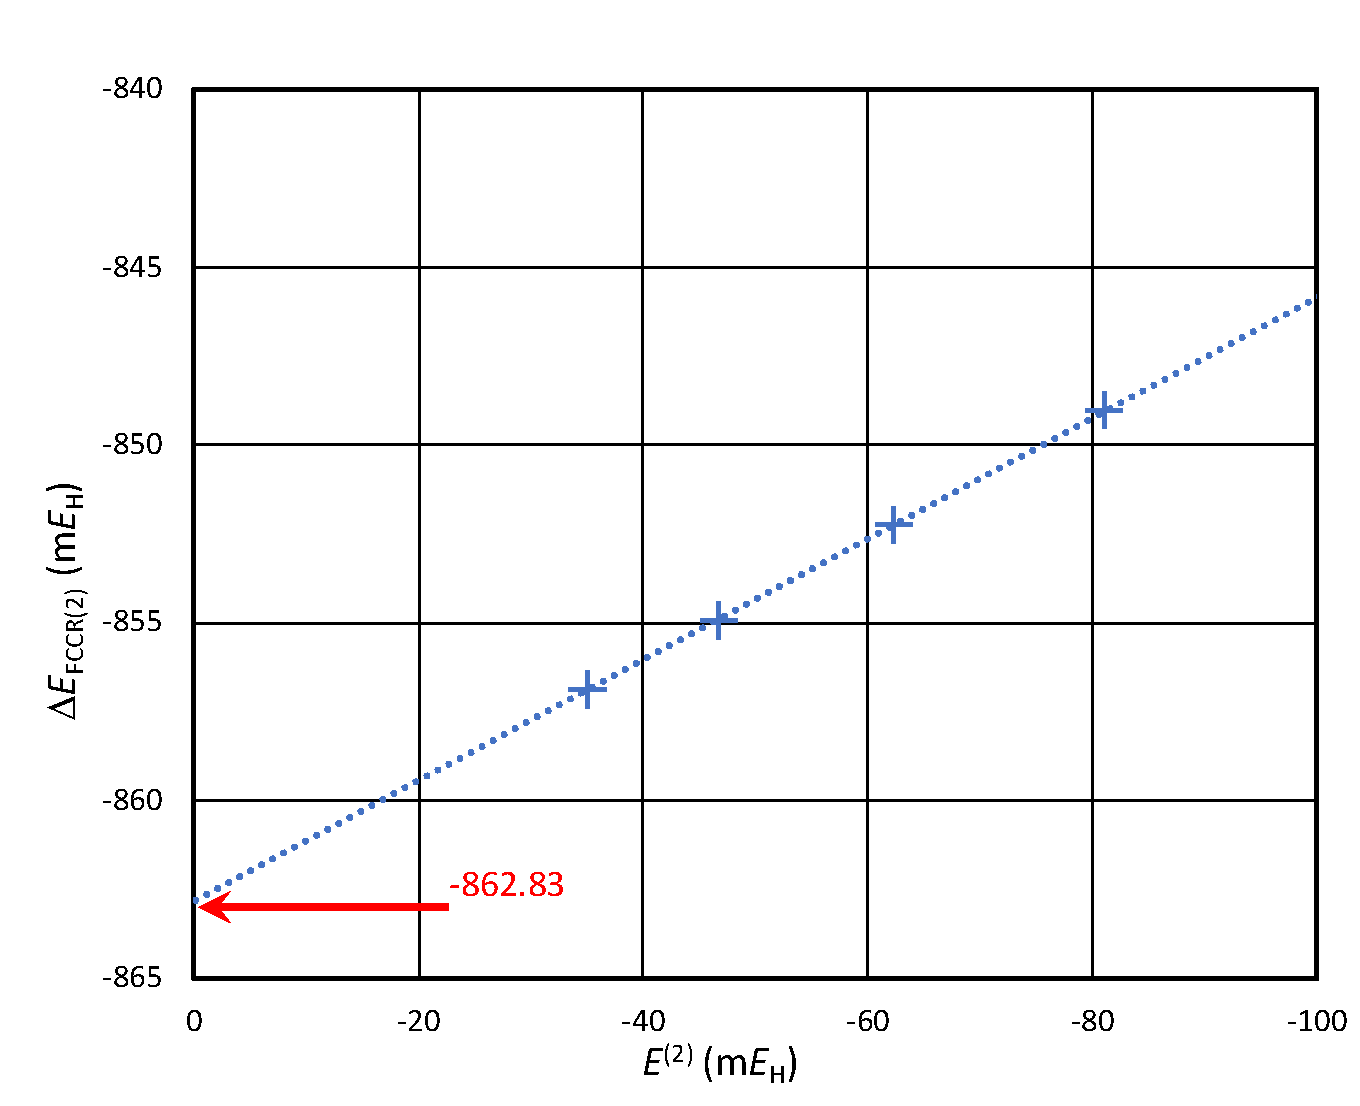
\includegraphics[scale=0.6]{figures/fccr/fccr.pdf}
\caption{Updated FCCR results. The linear extrapolation of the FCCR(2) energy.}
\label{fccr_updated_SI_fig}
\end{center}
\vspace{-0.6cm}
\end{figure}
%

\section{CCSDTQ}

The CCSDTQ~\cite{ccsdtq_paper_1_jcp_1991,ccsdtq_paper_2_jcp_1992} correlation energy of $\Delta E_{\text{CCSDTQ}} = -862.37$ m$E_{\text{H}}$ was obtained using the {\texttt{NCC}} module of the {\texttt{CFOUR}} program~\cite{matthews_stanton_ccsdtq_jcp_2015,ncc,cfour_paper,cfour} on a single Intel Xeon CPU E5-4620 node (8 cores $@$ 2.2 GHz, 15.0 GB/core). Convergence was reached in 10 iterations.

\section{Cluster Decomposition}

%
\begin{table}[ht!]
\begin{center}
\caption{Cluster decomposition ($L_2$-norm) of a 5M-determinant ASCI wave function (with delocalized orbitals) for excitation levels $1 \leq n \leq 6$.}
\label{cluster_decomp_SI_table}
\begin{tabular}{l|r|r|r}
\toprule
\multicolumn{1}{c|}{$n$} & \multicolumn{1}{c|}{$|\bm{c}_n|$} & \multicolumn{1}{c|}{$|\bm{t}_n|$} & \multicolumn{1}{c}{Ratio/$\%$} \\
\midrule\midrule
1 & $0.019477$ & $0.019477$ & $100.0$ \\
2 & $0.533103$ & $0.533108$ & $100.0$ \\
3 & $0.064742$ & $0.065137$ & $100.6$ \\
4 & $0.142888$ & $0.014178$ & $9.92$ \\
5 & $0.006201$ & $0.000465$ & $7.50$ \\
6 & $0.008792$ & $0.001948$ & $22.16$ \\
\midrule
\end{tabular}
\vspace{-0.6cm}
\end{center}
\end{table}
%
Table \ref{cluster_decomp_SI_table} presents results for a cluster decomposition~\cite{lehtola_head_gordon_fci_decomp_jcp_2017} of an ASCI wave function with $\num{5.e6}$ determinants (using delocalized orbitals, as described in Sec \ref{sec:asci}). These results indicate how most of the $\{\bm{c}_4\}$ (and higher order) CI coefficients comes from disconnected terms.\\

Subsequent to the main study, a cluster decomposition was also carried out on a $\num{4.e6}$ determinant ASCI wave function with localized orbitals (as described in Sec \ref{sec:asciloc}), as this CI wave function had a lower variational energy than the previous one ($-772$ m$E_{\text{H}}$ correlation vs $-737$ m$E_{\text{H}}$) and was thus a better approximation to the true FCI wave function. The resulting values are provided in Table \ref{cluster_decomp_SI_table2}, which differ slightly from those in Table \ref{cluster_decomp_SI_table}. The general picture however remains the same, in that $\{\bm{c}_4\}$ and higher order excitations seem to mostly arise from disconnected terms. 

\begin{table}[ht!]
	\begin{center}
		\caption{Cluster decomposition ($L_2$-norm) of a 4M-determinant ASCI wave function (with localized orbitals) for excitation levels $1 \leq n \leq 6$.}
		\label{cluster_decomp_SI_table2}
		\begin{tabular}{l|r|r|r}
			\toprule
			\multicolumn{1}{c|}{$n$} & \multicolumn{1}{c|}{$|\bm{c}_n|$} & \multicolumn{1}{c|}{$|\bm{t}_n|$} & \multicolumn{1}{c}{Ratio/$\%$} \\
			\midrule\midrule
			1&	$0.01777$ &	$0.01777$&	$100.0$\\
			2&	$0.55063$ &	$0.55063$&	$100.0$\\
			3&	$0.06855$ &	$0.06868$&	$100.2$\\
			4&	$0.16486$ &	$0.01755$&	$10.65$\\
			5&	$0.00903$ &	$0.00076$&	$8.38$\\
			6&	$0.01610$ &	$0.00259$&	$16.11$\\
			\midrule
		\end{tabular}
		\vspace{-0.6cm}
	\end{center}
\end{table}


\newpage

\bibliography{si.bib}

%
\end{document}
